\documentclass[a4paper]{article}

\usepackage[utf8]{inputenc}
\usepackage[T1]{fontenc}
\usepackage{textcomp}
\usepackage[UKenglish]{babel}
\usepackage{amsmath, amssymb}
\usepackage{subcaption}
\usepackage{listings}
\usepackage{float}

\setlength{\parindent}{0pt}
\setlength{\parskip}{1em}


% figure support
\usepackage{import}
\usepackage{xifthen}
\pdfminorversion=7
\usepackage{pdfpages}
\usepackage{transparent}
\newcommand{\incfig}[1]{%
	\def\svgwidth{\columnwidth}
	\import{./figures/}{#1.pdf_tex}
}

\pdfsuppresswarningpagegroup=1

\begin{document}
	\section{Part 1: Thresholding}
	\subsection{Introduction}
	Thresholding is a technique used to segment an image based on grey level
	intensities within the image. Two common methods of thresholding an
	image are applying a "Fixed Global Threshold" and applying an "Adaptive
	Threshold". Each of these methods take a greyscale input image, and
	output a binary (black and white) image.
	\par Fixed Global thresholding involves applying a single threshold value
	across the image, i.e. if the intensity value of the pixel is greater
	than the threshold value, set that pixel to white, otherwise, set it to
	black.
	\par Adaptive thresholding techniques base their threshold values at the
	current pixel off the neighbouring pixels. The "5x5 Adaptive
	Thresholding" method utilised in this section takes the mean intensity
	value of the 24 pixels surrounding the currently selected pixel as the
	threshold value for the currently selected pixel. If this center pixels
	intensity value is greater than the threshold, it's value is set to
	white, otherwise it is set to black.
	\subsection{Techniques}
	In completing this section of the assignment, the following techniques
	are utilised:
	\subsubsection{Part a}
	\underline{\textbf{Load Image}}
	\par Matlabs ``imread()'' function is used to load an image, whose filename
	is passed as an argument to the function, as an array in the form
	$X \times Y \times 3$ where X and Y are the dimensions of the image, and
	the ``3'' represents the colour channels (RGB).
	\par \underline{\textbf{Colour to Greyscale}}
	\par The Matlab ``rgb2gray()'' function converts a colour image to a
	greyscale image. The three channel RGB image is converted to a single
	channel greyscale image based on the luminance of each pixel in the
	image. The output single channel values range from $0-255$.
	\par\underline{\textbf{Show Image}}
	\par The Matlab ``imshow()'' function is used to display an image on
	screen.
	\subsubsection{Part b}
	\underline{\textbf{Threshold}}
	\par The VSG ``Threshold'' function applies a fixed global threshold to
	the input image. If the pixel value is less than the threshold value,
	the pixel is set to black, otherwise it is set to white.
	\subsubsection{Part c}
	\underline{\textbf{5x5 Threshold}}
	\par The VSG ``5x5Thresh'' function applies an adaptive 5x5 threshold
	to the image. The function defaults to a threshold offset of value zero.
	\par When the value of the center pixel in the 5x5 region is less than the
	mean of the 5x5 region minus the offset, the pixel is set to black,
	otherwise it is set to white.
	\subsubsection{Part d}
	\underline{\textbf{Gaussian Noise}}
	The Matlab ``imnoise()'' function, when used with the `gaussian' input
	parameter, applies Gaussian noise with mean specified by input
	parameter `m', and variance `var', e.g:
	\begin{lstlisting}
	imnoise(img1, 'gaussian', 0, var)
	\end{lstlisting}
	The above example applies zero-mean Gaussian noise to the image
	``img1'', with a variance ``var''.
	\subsection{Pseudocode}
	\subsubsection{Part a}
	\begin{enumerate}
		\item Load the image into Matlab using the ``imread()''
			function
		\item Use the ``rgb2gray()'' function to convert the image to
			greyscale.
		\item Display the greyscale image using the ``imshow()''
			function.
	\end{enumerate}
	\subsubsection{Part b}
	\begin{enumerate}
		\item Follow the steps of Part a.
		\item Apply a fixed global threshold using the VSG package
			``Threshold'' function. An arbitrary value should be
			chosen for the fixed threshold value.
		\item Vary the fixed threshold value in order to obtain optimal
			background/foreground segmentation, while retaining
			facial features.
		\item Display the thresholded images using the ``imshow()''
			function.
	\end{enumerate}
	\subsubsection{Part c}
	\begin{enumerate}
		\item Follow the steps of Part a.
		\item Apply a 5x5 adaptive threshold using the VSG package
			"5x5Thresh" function.
		\item Display the adaptive thresholded image using the
			``imshow()'' function.
	\end{enumerate}
	\subsubsection{Part d}
	\begin{enumerate}
		\item Follow the steps of Part a.
		\item Apply Gaussian noise to the greyscale image using the MIP
			``imnoise()'' function. Zero-mean noise should be used
			for this section.
		\item Execute the fixed global thresholding and 5x5 adaptive
			thresholding procedures as described in part b and part
			c respectively.
		\item Adjust the variance value of the ``imnoise()'' function.
			Repeat steps 2 and 3.
	\end{enumerate}
	\subsection{Results}
	\subsubsection{Part a}
	The image is correctly loaded into Matlab, converted to greyscale, and
	displayed. The input image is of dimensions $512\times 348\times 3$, and
	is of data type integer. This means that the image is in the RGB colour
	space, with the red, green, and blue channels represented by a value of
	0-255 for each pixel in the image. The resulting greyscale image is of
	dimensions  $512\times 384$ and is also of type integer. The single
	channel representing the greyscale intensities have values ranging from
	0-255.
	\begin{figure}[H]
		\centering
		\subcaptionbox{Input Image}
		[.3\linewidth]{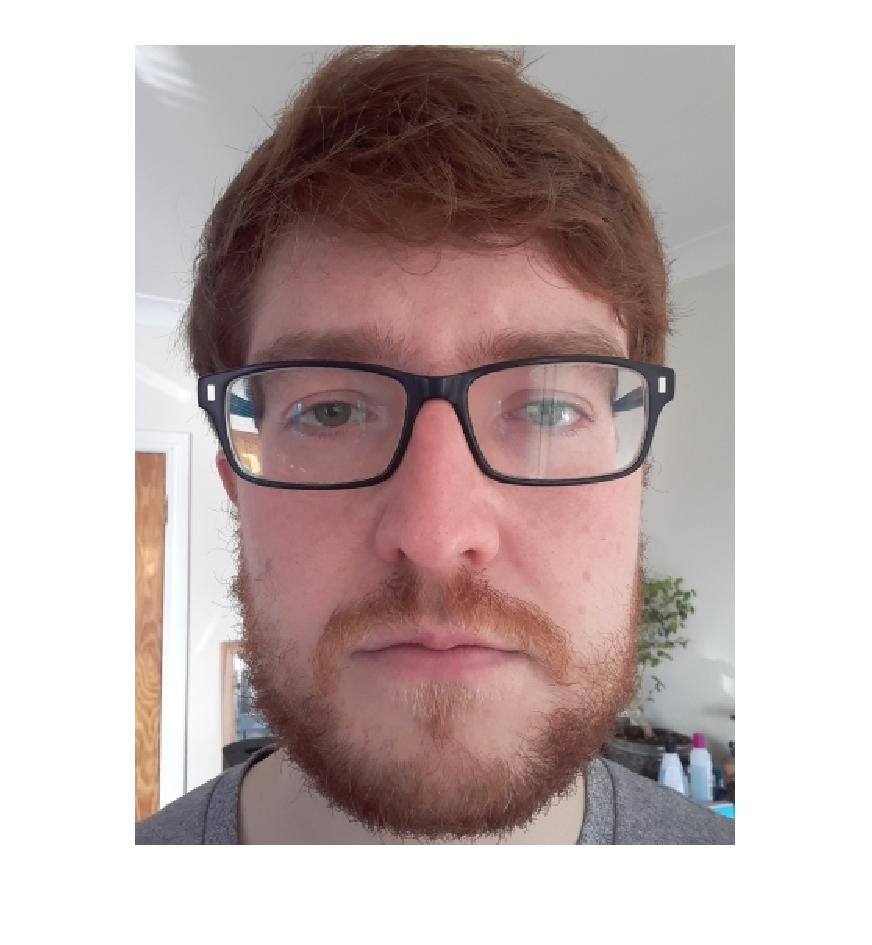
\includegraphics[height=5cm]{Results/Q1/a/qaInput.jpg}}%
		\subcaptionbox{Greyscale Image}
		[.3\linewidth]{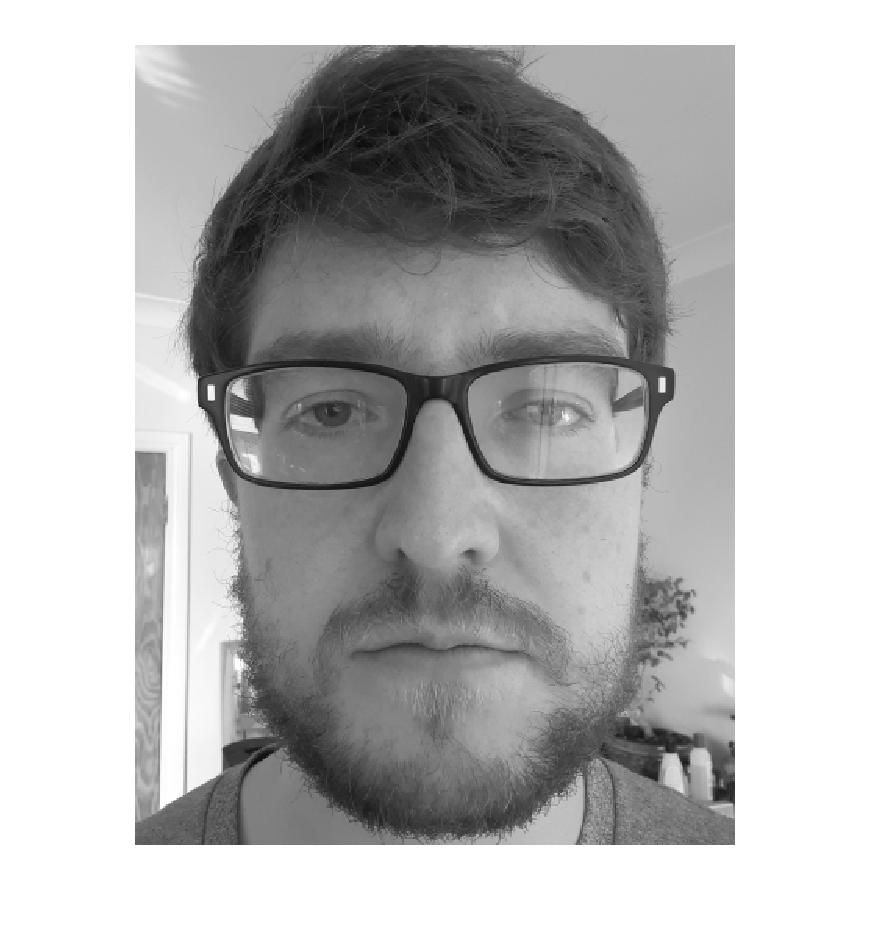
\includegraphics[height=5cm]{Results/Q1/a/qaGreyscale.jpg}}%
		\caption{Input and Greyscale Images}
		\label{fig:}
	\end{figure}
	\subsubsection{Part b}
	The VSG ``Threshold'' function is applied, with varying threshold
	values, to the input greyscale image. The ``Threshold'' function returns
	images with the same dimensions as the input image, however the data
	type returned is ``double'' rather than ``integer''. The initial value of the
	threshold is 199, calculated by taking !!!!!!!!!. As this threshold does not
	provide adequate separation of the features in the image, arbitrary
	values of 125, 130, and 140 are also used. The image thresholded at 125
	has the greatest level of separation between the face and background,
	while also retaining as much detail as possible in the facial features.
	\begin{figure}[H]
		\centering
		\subcaptionbox{Data Driven Threshold}
		[.3\linewidth]{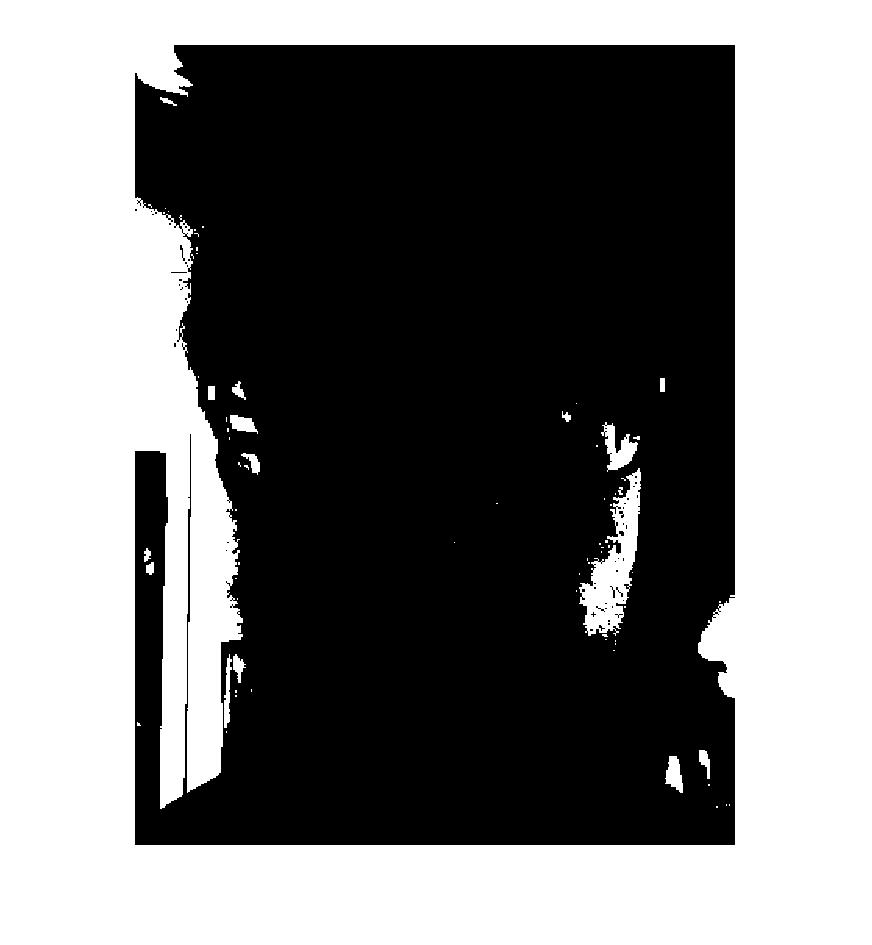
\includegraphics[height=5cm]{Results/Q1/b/qbThreshData.jpg}}%
		\subcaptionbox{Threshold$=125$}
		[.3\linewidth]{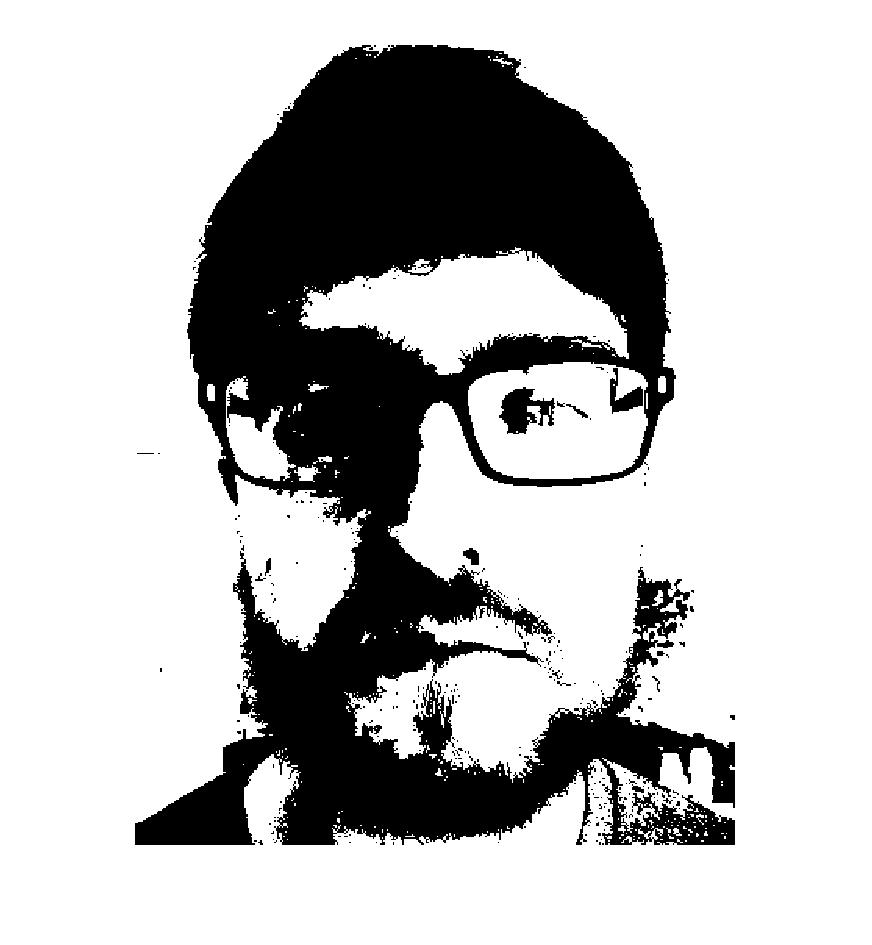
\includegraphics[height=5cm]{Results/Q1/b/qbThresh125.jpg}}%
		\caption{``Threshold'' Function Output}
		\label{fig:}
	\end{figure}
	\begin{figure}[H]
		\centering
		\subcaptionbox{Threshold$=130$}
		[.3\linewidth]{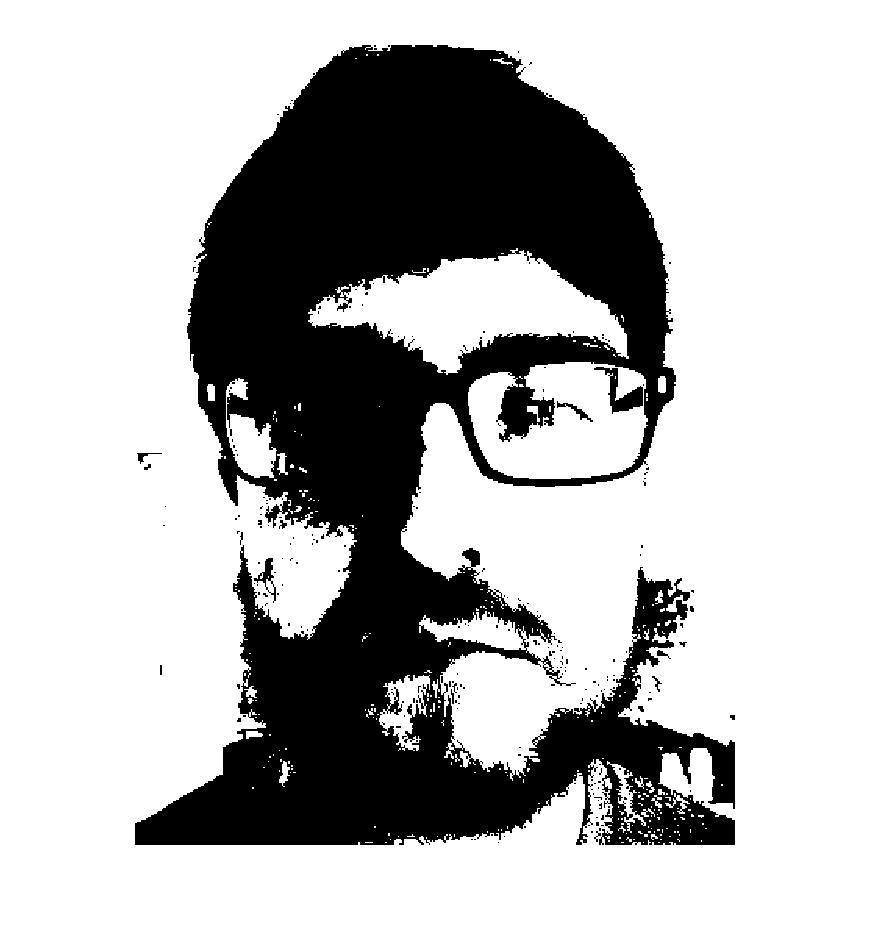
\includegraphics[height=5cm]{Results/Q1/b/qbThresh130.jpg}}%
		\subcaptionbox{Threshold$=140$}
		[.3\linewidth]{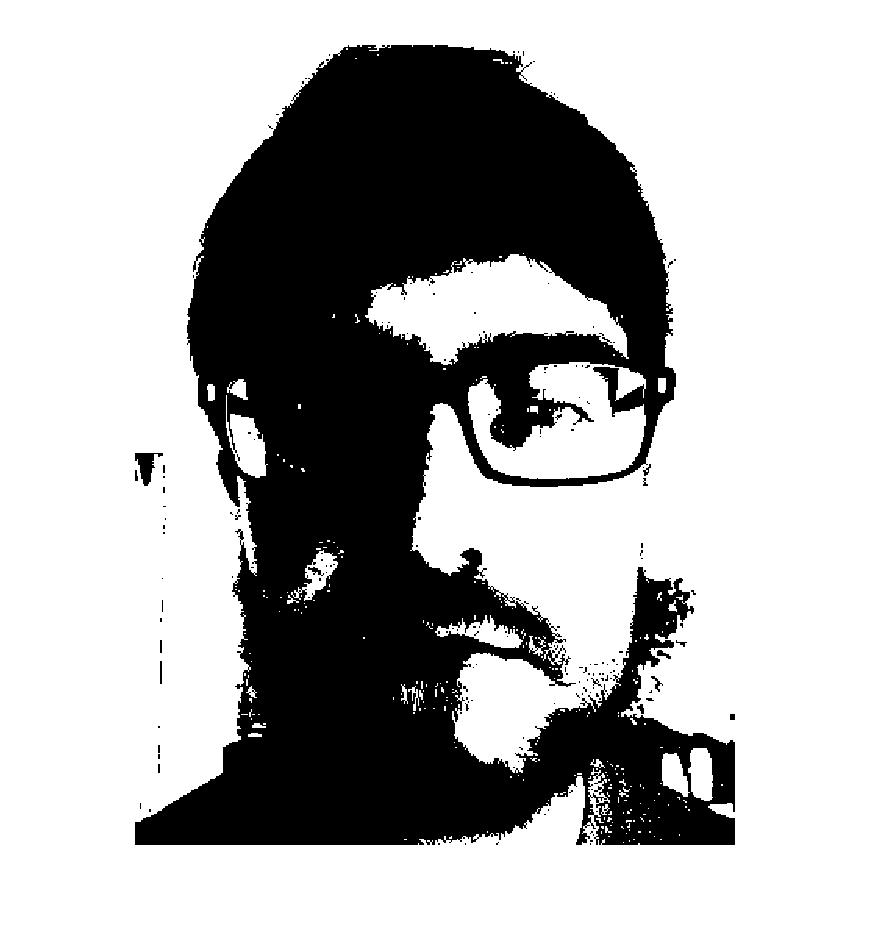
\includegraphics[height=5cm]{Results/Q1/b/qbThresh140.jpg}}%
		\caption{``Threshold'' Function Output}
		\label{fig:}
	\end{figure}
	\subsubsection{Part c}
	The VSG ``5x5Thresh'' function is applied to the input greyscale image.
	The resulting image is of type ``double'' and has the same dimensions as
	the input image. When compared with the fixed global threshold images,
	there is much greater separation of the foreground from the background,
	with all of the facial features fully visible. Features which are
	thresholded out due to lighting conditions in the fixed global threshold
	are retained here, such as the eyes.
	\begin{figure}[H]
		\centering
		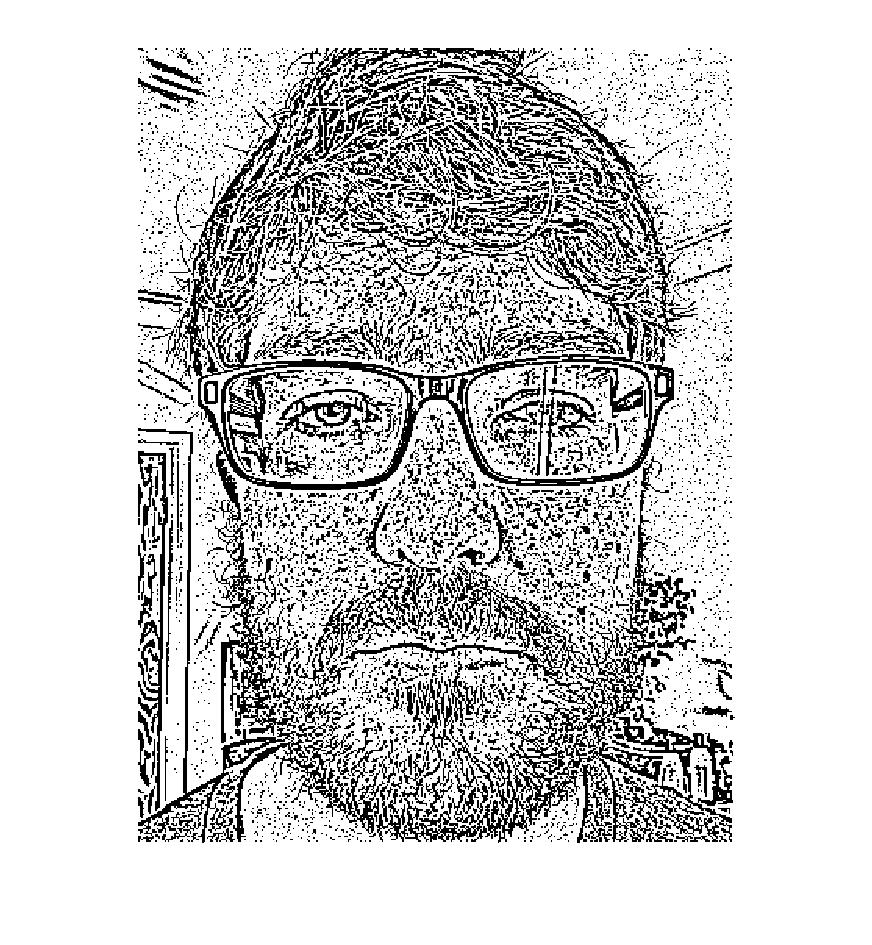
\includegraphics[height=5cm]{Results/Q1/c/qcThresh5x5.jpg}%
		\caption{``5x5Thresh'' Function Output}
		\label{fig:}
	\end{figure}
	\subsubsection{Part d}
	Gaussian noise is added to the greyscale image, and the ``Threshold''
	and ``5x5Thresh'' functions are applied. As can be observed from the
	images, the fixed global threshold is less sensitive to noise. This is
	due to the 5x5 Threshold using the average value of an area of pixels to
	set the threshold value. As such, noise within an area can skew the
	result of the thresholding, making this function much more sensitive
	to noise.
	\begin{figure}[H]
		\centering
		\subcaptionbox{Noisy Image}
		[.3\linewidth]{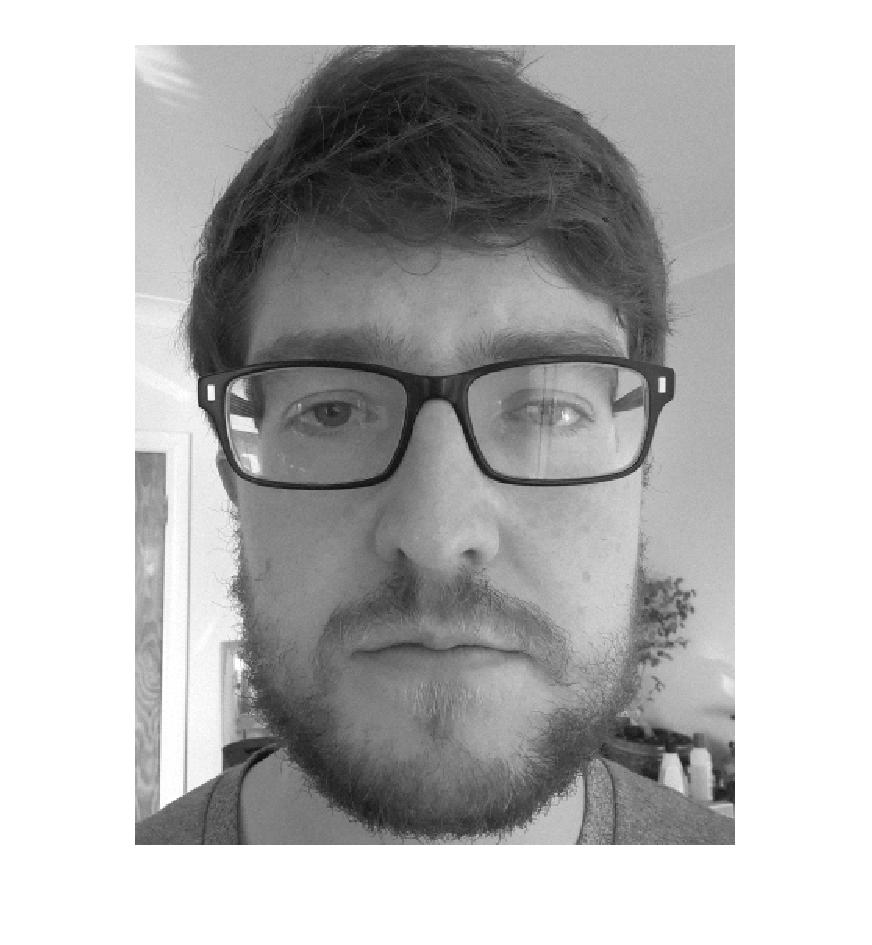
\includegraphics[height=5cm]{Results/Q1/d/qdVar00001.jpg}}%
		\subcaptionbox{Global Threshold}
		[.3\linewidth]{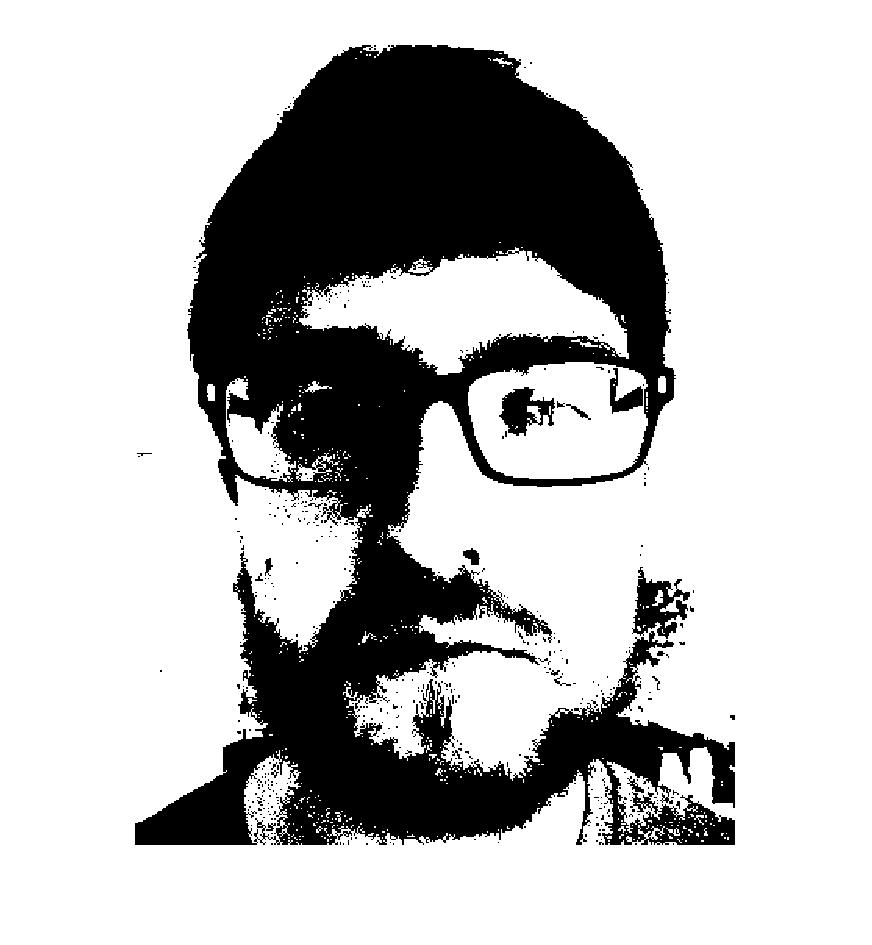
\includegraphics[height=5cm]{Results/Q1/d/qdThresh00001.jpg}}%
		\subcaptionbox{5x5 Threshold}
		[.3\linewidth]{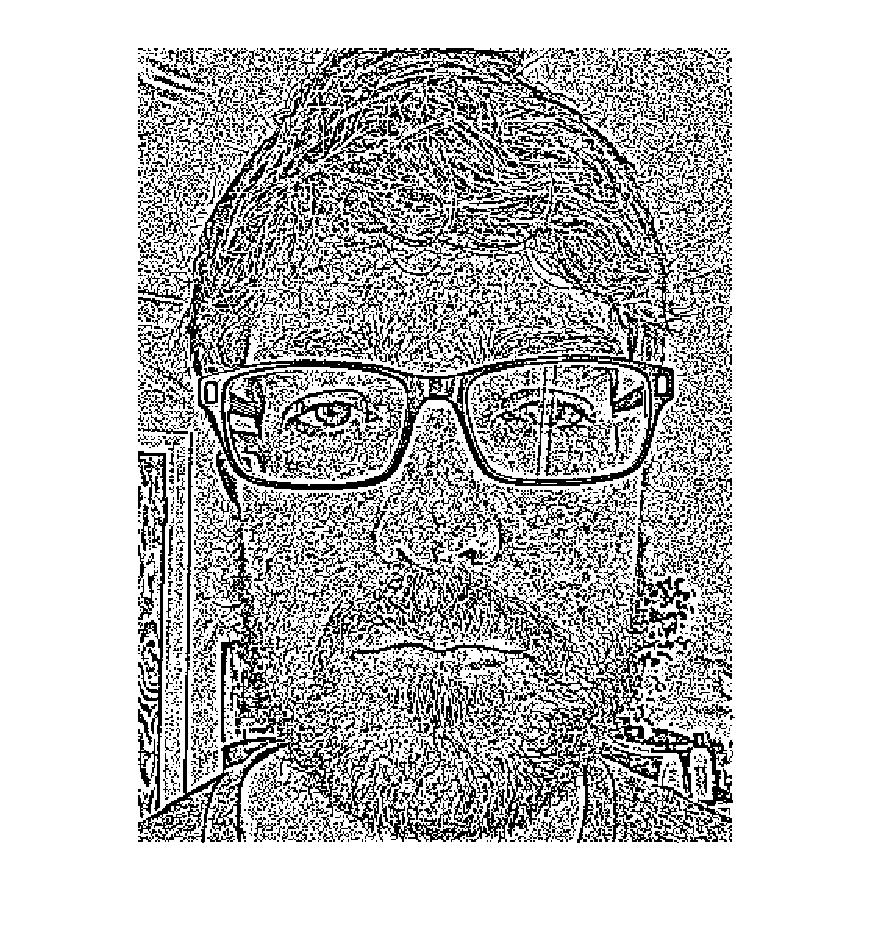
\includegraphics[height=5cm]{Results/Q1/d/qd5x500001.jpg}}%
		\caption{Thresholded Images after Gaussian Noise (0.0001
		Variance)}
		\label{fig:}
	\end{figure}
	\begin{figure}[H]
		\centering
		\subcaptionbox{Noisy Image}
		[.3\linewidth]{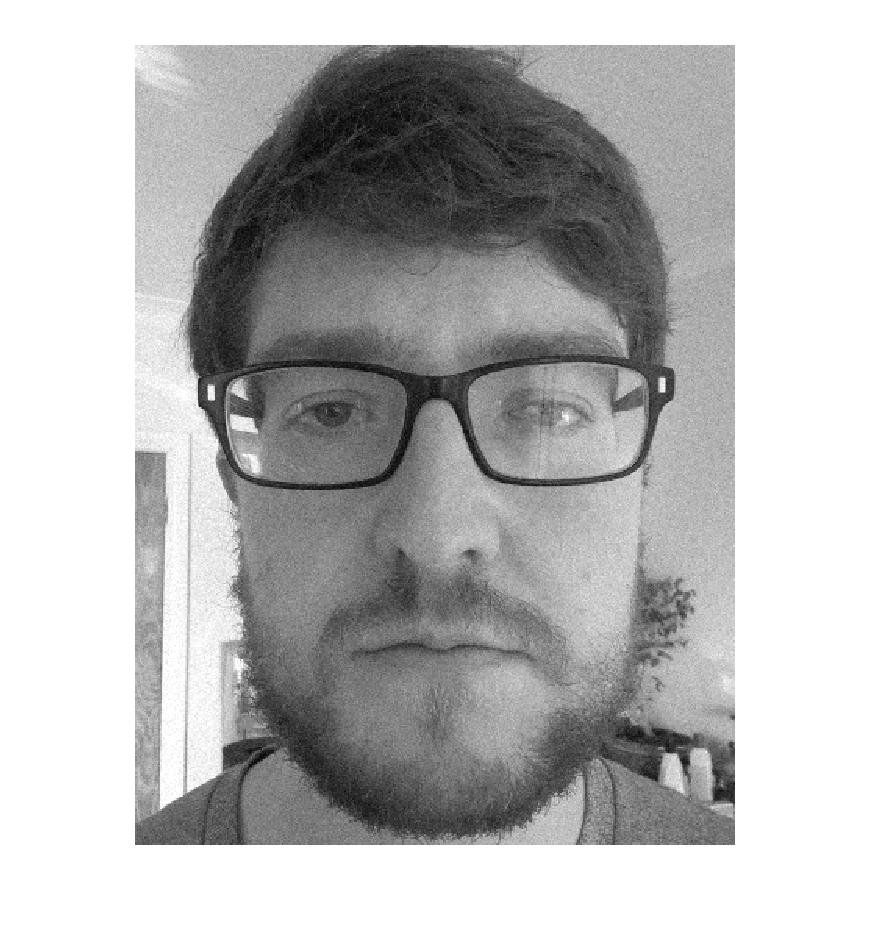
\includegraphics[height=5cm]{Results/Q1/d/qdVar0001.jpg}}%
		\subcaptionbox{Global Threshold}
		[.3\linewidth]{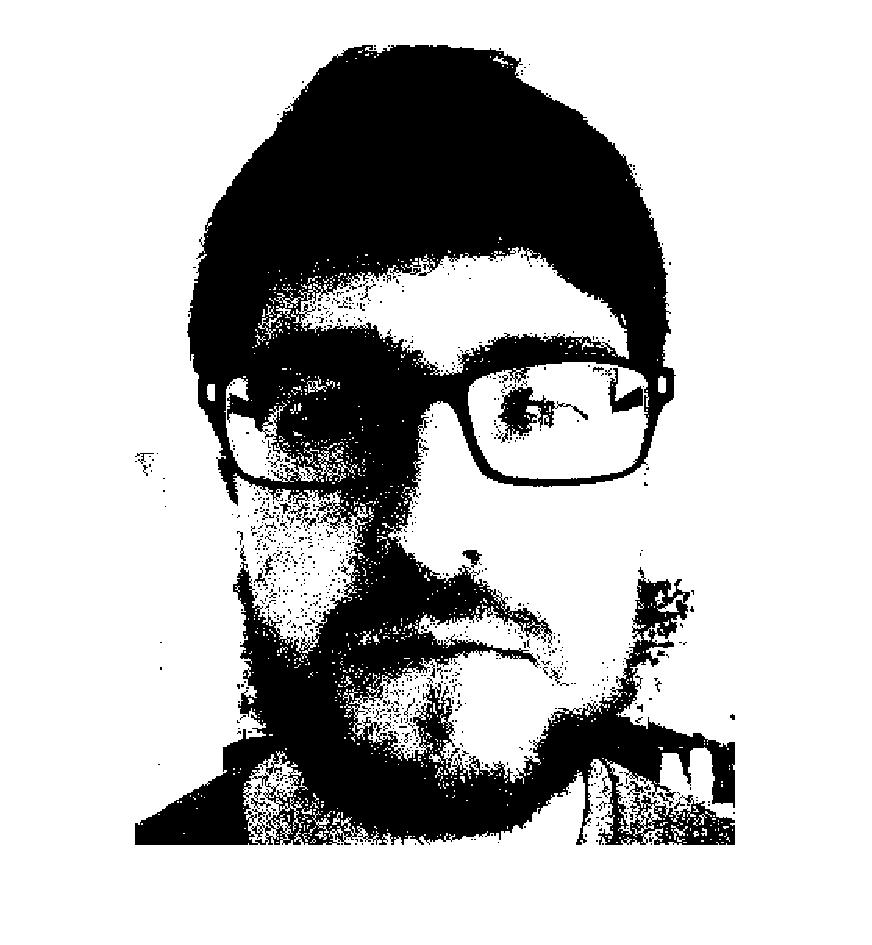
\includegraphics[height=5cm]{Results/Q1/d/qdThresh0001.jpg}}%
		\subcaptionbox{5x5 Threshold}
		[.3\linewidth]{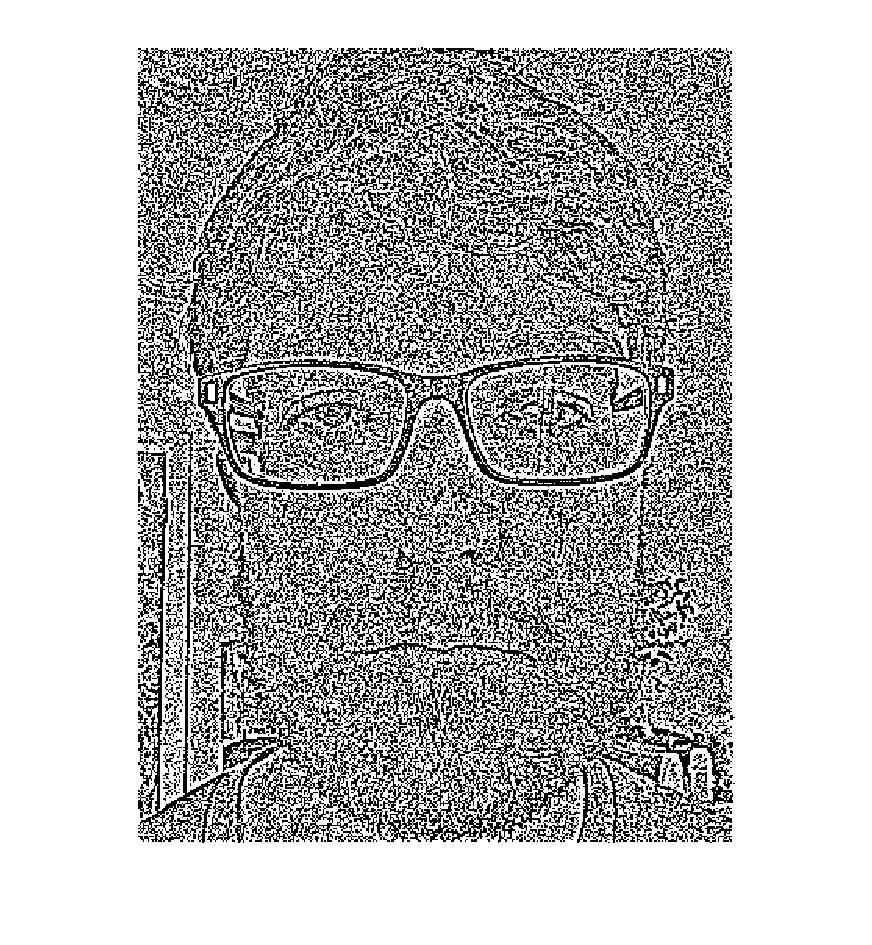
\includegraphics[height=5cm]{Results/Q1/d/qd5x50001.jpg}}%
		\caption{Thresholded Images after Gaussian Noise (0.001 Variance)}
		\label{fig:}
	\end{figure}
	\begin{figure}[H]
		\centering
		\subcaptionbox{Noisy Image}
		[.3\linewidth]{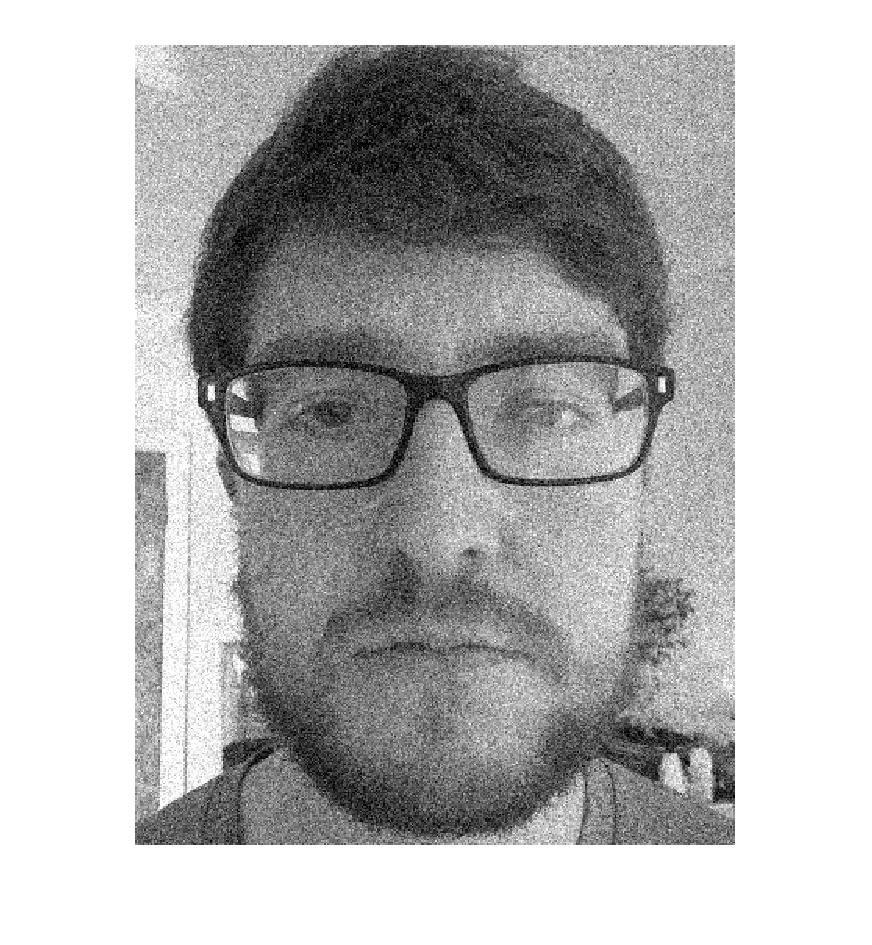
\includegraphics[height=5cm]{Results/Q1/d/qdVar001.jpg}}%
		\subcaptionbox{Global Threshold}
		[.3\linewidth]{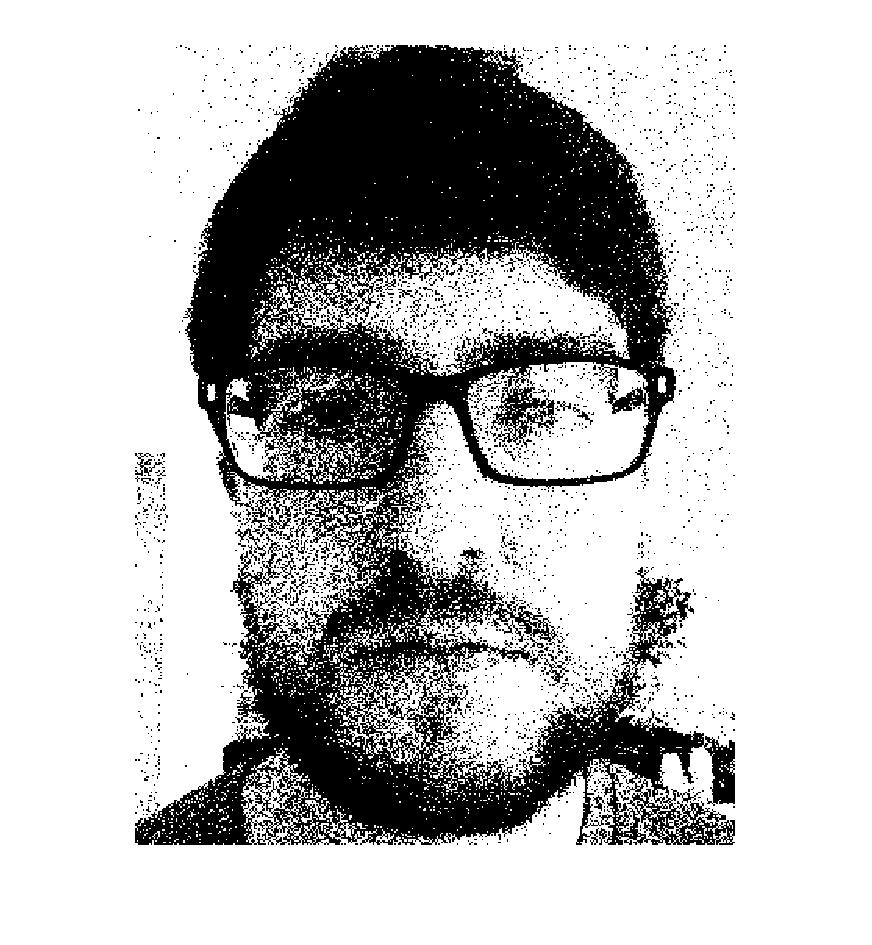
\includegraphics[height=5cm]{Results/Q1/d/qdThresh001.jpg}}%
		\subcaptionbox{5x5 Threshold}
		[.3\linewidth]{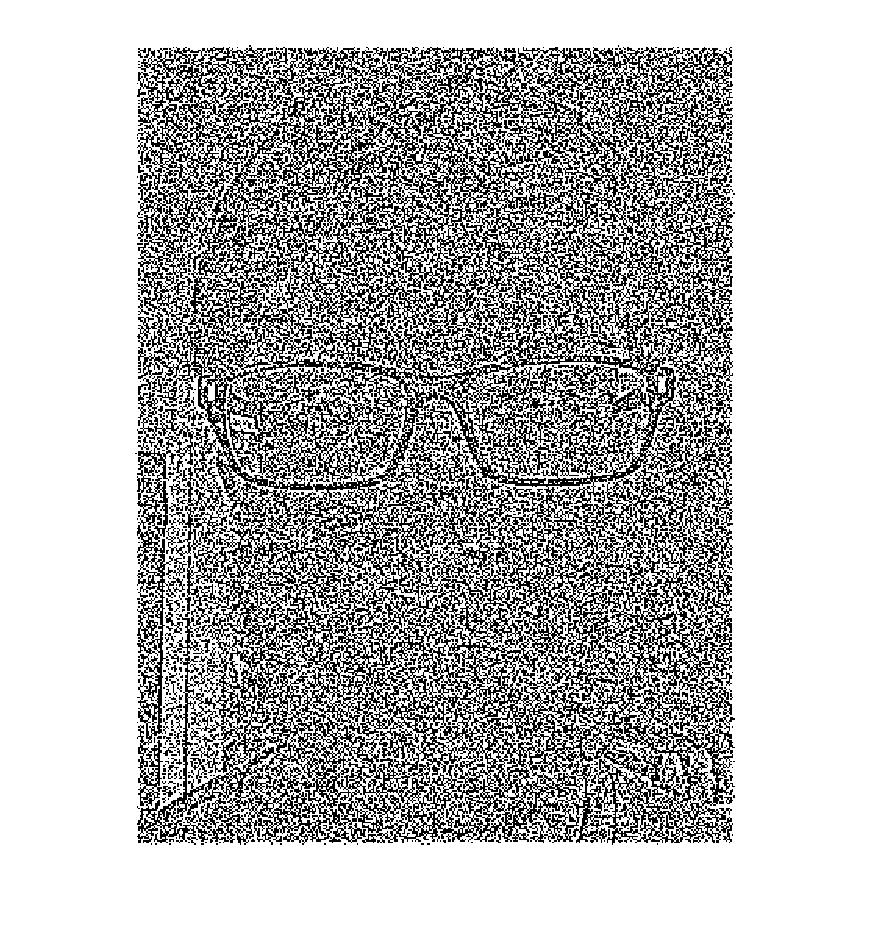
\includegraphics[height=5cm]{Results/Q1/d/qd5x5001.jpg}}%
		\caption{Thresholded Images after Gaussian Noise (0.01 Variance)}
		\label{fig:}
	\end{figure}
	\begin{figure}[H]
		\centering
		\subcaptionbox{Noisy Image}
		[.3\linewidth]{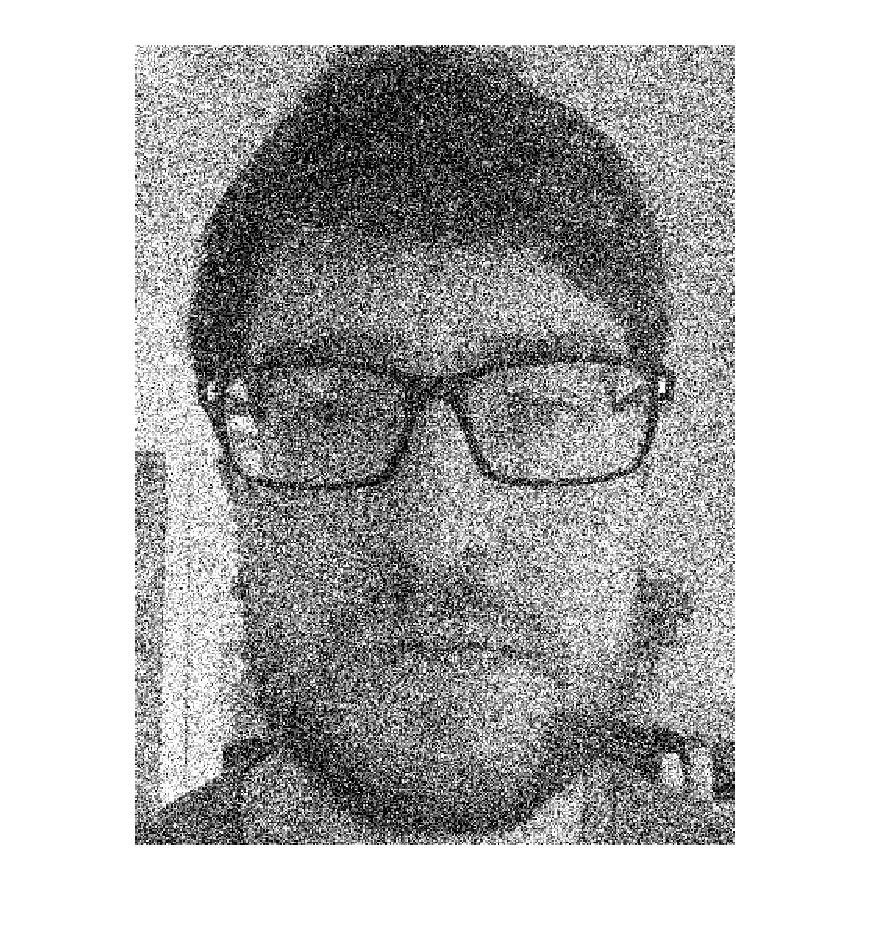
\includegraphics[height=5cm]{Results/Q1/d/qdVar01.jpg}}%
		\subcaptionbox{Global Threshold}
		[.3\linewidth]{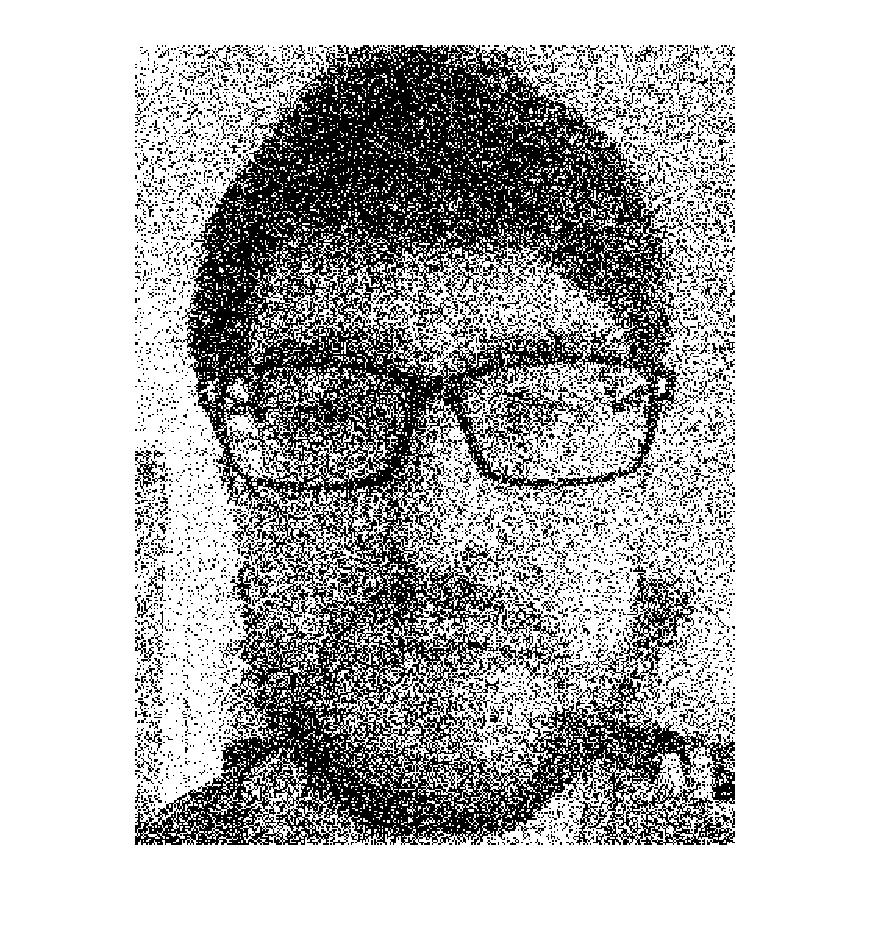
\includegraphics[height=5cm]{Results/Q1/d/qdThresh01.jpg}}%
		\subcaptionbox{5x5 Threshold}
		[.3\linewidth]{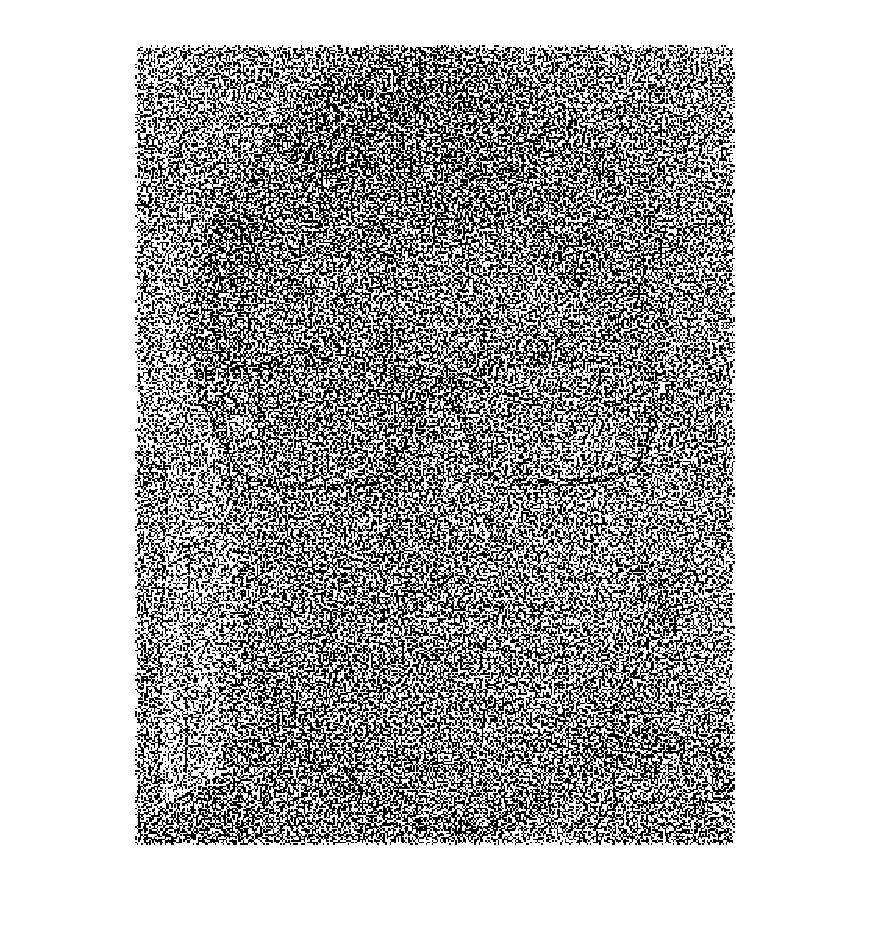
\includegraphics[height=5cm]{Results/Q1/d/qd5x501.jpg}}%
		\caption{Thresholded Images after Gaussian Noise (0.1 Variance)}
		\label{fig:}
	\end{figure}
	\begin{figure}[H]
		\centering
		\subcaptionbox{Noisy Image}
		[.3\linewidth]{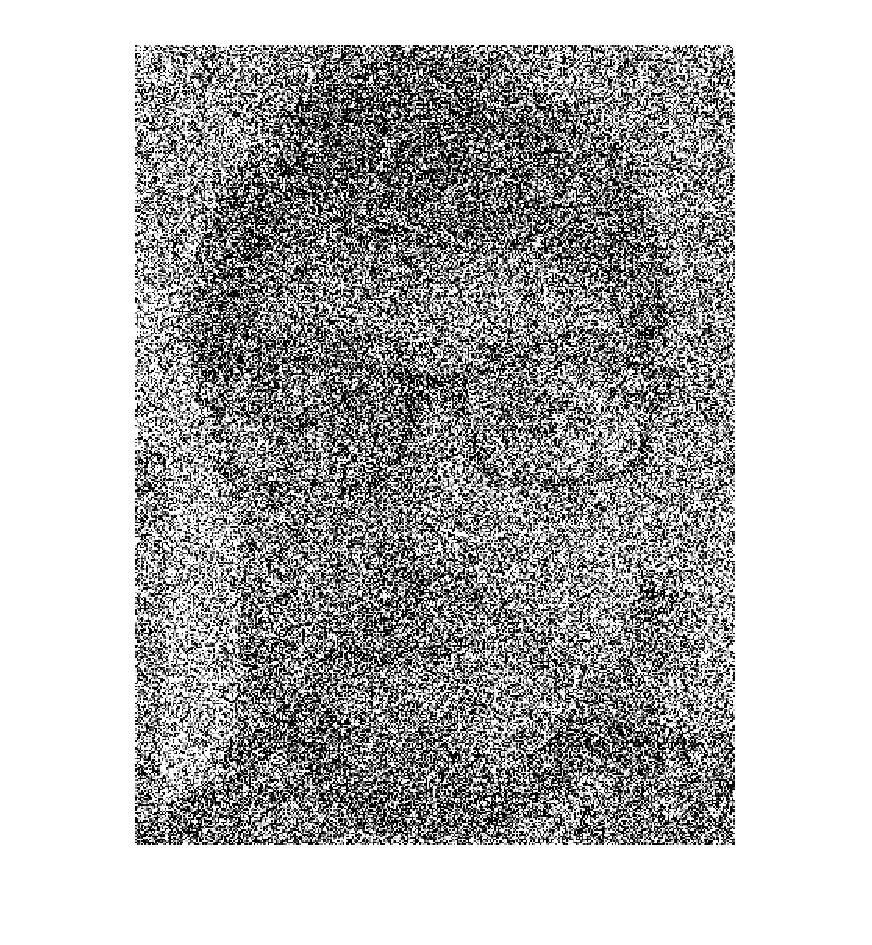
\includegraphics[height=5cm]{Results/Q1/d/qdVar1.jpg}}%
		\subcaptionbox{Global Threshold}
		[.3\linewidth]{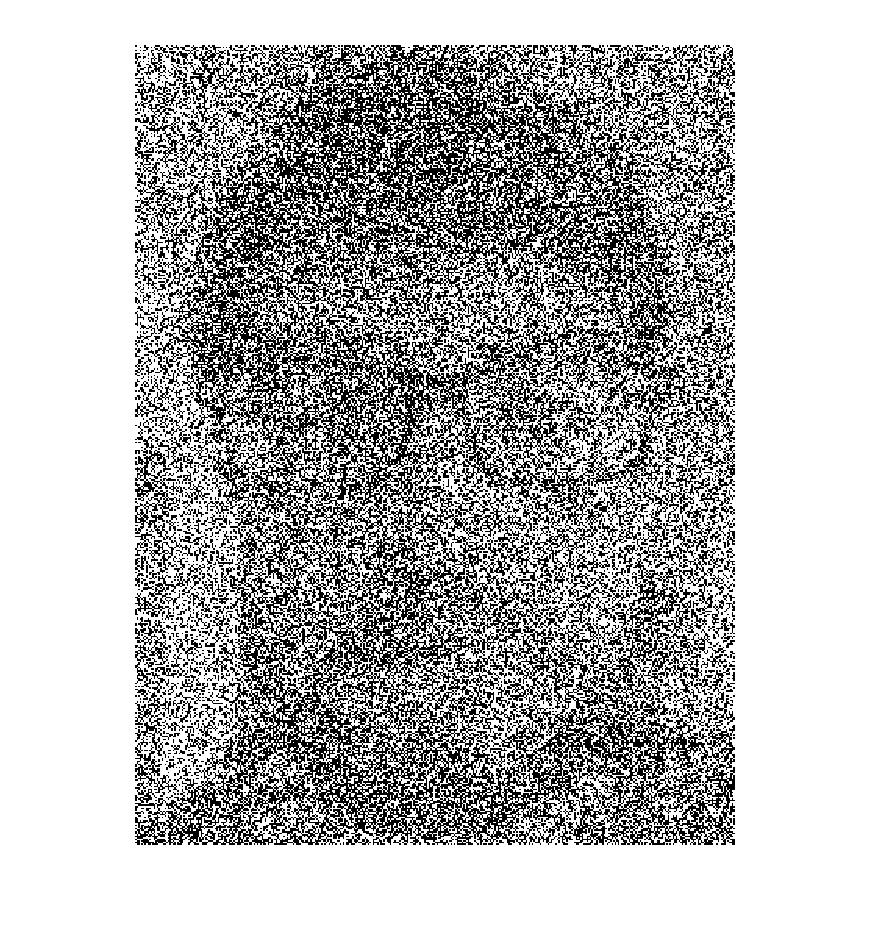
\includegraphics[height=5cm]{Results/Q1/d/qdThresh1.jpg}}%
		\subcaptionbox{5x5 Threshold}
		[.3\linewidth]{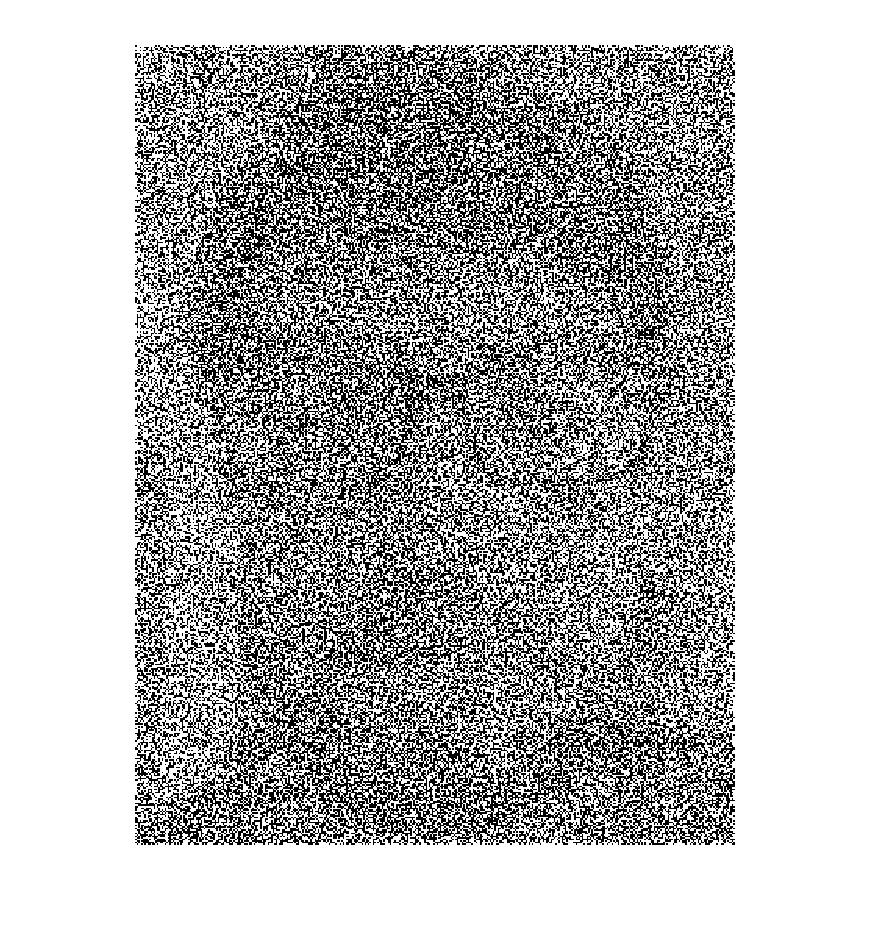
\includegraphics[height=5cm]{Results/Q1/d/qd5x51.jpg}}%
		\caption{Thresholded Images after Gaussian Noise (1 Variance)}
		\label{fig:}
	\end{figure}
	\par It can be seen that until a variance of approximately
	\subsection{Conclusion}
	\section{Part 2: Segmentation}
	\subsection{Introduction}
	Segmentation is the practice of extracting features from an image. In
	this section, the main alphanumeric registration characters of a licence
	plate must be extracted from the overall image. The extracted characters
	must not include either the country code, county name, or dashes between
	sections of the registration.
	\par Automated and data driven segmentation can be achieved by combining
	arithmetic functions and blob functions. As the size ratio of each letter in
	the registration does not change with scale, this ratio can be utilised
	to remove only blobs under a size specified by the largest letter
	(blob).
	\subsection{Techniques}
	\subsubsection{Part a}
	\underline{\textbf{Low Pass Filter}}
	\par The VSG ``LowPass'' filter function applies a 3x3 low pass filter
	to the image.
	\par\underline{\textbf{Mid-Threshold}}
	\par Much like the aforementioned ``Threshold'' function, the
	``MidThresh'' function applies a single threshold value to the image.
	The threshold value chosen is 125, the middle of the 0-255 range of the
	integer input values.
	\par\underline{\textbf{Inversion (NOT)}}
	\par Inversion is achieved using the VSG ``NOT'' function, which
	performs a boolean Not operation on each pixel of the image. On a binary
	image, this changes all white pixels to black, and all black pixels to
	white.
	\par\underline{\textbf{Biggest Blob}}
	\par The ``BiggestBlob'' function of the VSG toolbox outputs an image
	containing only the biggest single white blob from the binary input
	image.
	\par\underline{\textbf{Subtract}}
	\par The VSG ``Subtract'' function performs matrix subtraction between the
	specified images. Each pixel of the input image has its value
	subtracted from the corresponding pixel in the other image. As in this
	section, if one	image is binary, and the other RGB colour, the binary
	image is subtracted from the red channel of the RGB image.
	\par\underline{\textbf{White Pixel Counter}}
	\par The VSG ``WPCounter'' function counts the number of white pixels
	within the input image, outputting its value as an integer.
	\par\underline{\textbf{Mask}}
	\par The VSG ``MaskImg'' function applies a border mask of the input
	thickness to the image. The masked pixels which fall within the
	thickness have their values set to 0 (black).
	\par\underline{\textbf{Exclusive Or (XOR)}}
	\par The Exclusive Or function is completed using the VSG ``XOR''
	function. A bitwise XOR operation applied to binary images returns a
	white pixel only if the pixel is white in exactly one of the two input
	images.
	\par\underline{\textbf{Count Blobs}}
	The ``CountBlobs'' function of the VSG toolbox counts the number of
	white blobs in the input image, outputting its value as an integer.
	\par\underline{\textbf{Canny}}
	\par The VSG ``Canny'' edge detection function returns the image with
	any edges highlighted.
	\par\underline{\textbf{Add}}
	\par The VSG ``Add'' function performs matrix addition between the
	specified images. Each pixel of the input image has its value added to
	the corresponding pixel in the other image. As in this section, if one
	image is binary, and the other RGB colour, the binary image is added to
	the red channel of the RGB image.
	\subsection{Pseudocode}
	\subsubsection{Part a}
	\begin{enumerate}
		\item Load the image into Matlab using the ``imread()''
			function
		\item Use the ``rgb2gray()'' function to convert the image to
			greyscale.
		\item Display the greyscale image using the ``imshow()''
			function.
		\item Apply a low pass filter, using the VSG ``LowPass'' function,
			to remove noise from the image.
		\item Apply a threshold to the image using the VSG
			``MidThreshold'' function.
		\item Invert the image using the VSG ``NOT'' function.
		\item Extract the biggest blob (Country code and outer border),
			using the ``BiggestBlob'' VSG function.
		\item Subtract the extracted biggest blob image from the original
			image using the VSG ``Subtract'' function.
		\item Extract the biggest blob, using the ``BiggestBlob''
			function, (the largest alphanumeric character in the
			registration) .
		\item Using the VSG package ``WPCounter'' function, count the
			number of pixels in the biggest blob.
		\item Apply a single pixel mask to the image in order to remove
			the white pixel border.
		\item Compare the next biggest blob with the biggest blob, if
			the size is within the given ratio, ``XOR'' this with the
			image containing the previous biggest blob. Subtract
			this blob from the original image to avoid unintended
			looping. Repeat until the blob checked does not match
			the given ratio.
		\item Count the number of blobs in the resulting image using the
			VSG ``CountBlobs'' function.
		\item Use the VSG 'Canny' function to output an edge detector
			representation of the extracted characters.
		\item Overlay the resulting image on the original input image
			using the VSG 'Add' function.
	\end{enumerate}
	\subsubsection{Part b}
	\begin{enumerate}
		\item Apply ``imnoise()'' to the greyscale image, repeating the
			steps in part a.
		\item Increase the variance until the incorrect output value is
			acquired.
	\end{enumerate}
	\subsection{Results}
	\subsubsection{Part a}
	In part a, the alphanumeric registration characters of the licence plate
	are correctly extracted. The licence plate image is first loaded into
	Matlab, converted to greyscale, and a low pass filter is applied.
	\begin{figure}[H]
		\centering
		\subcaptionbox{Input Image}
		[.3\linewidth]{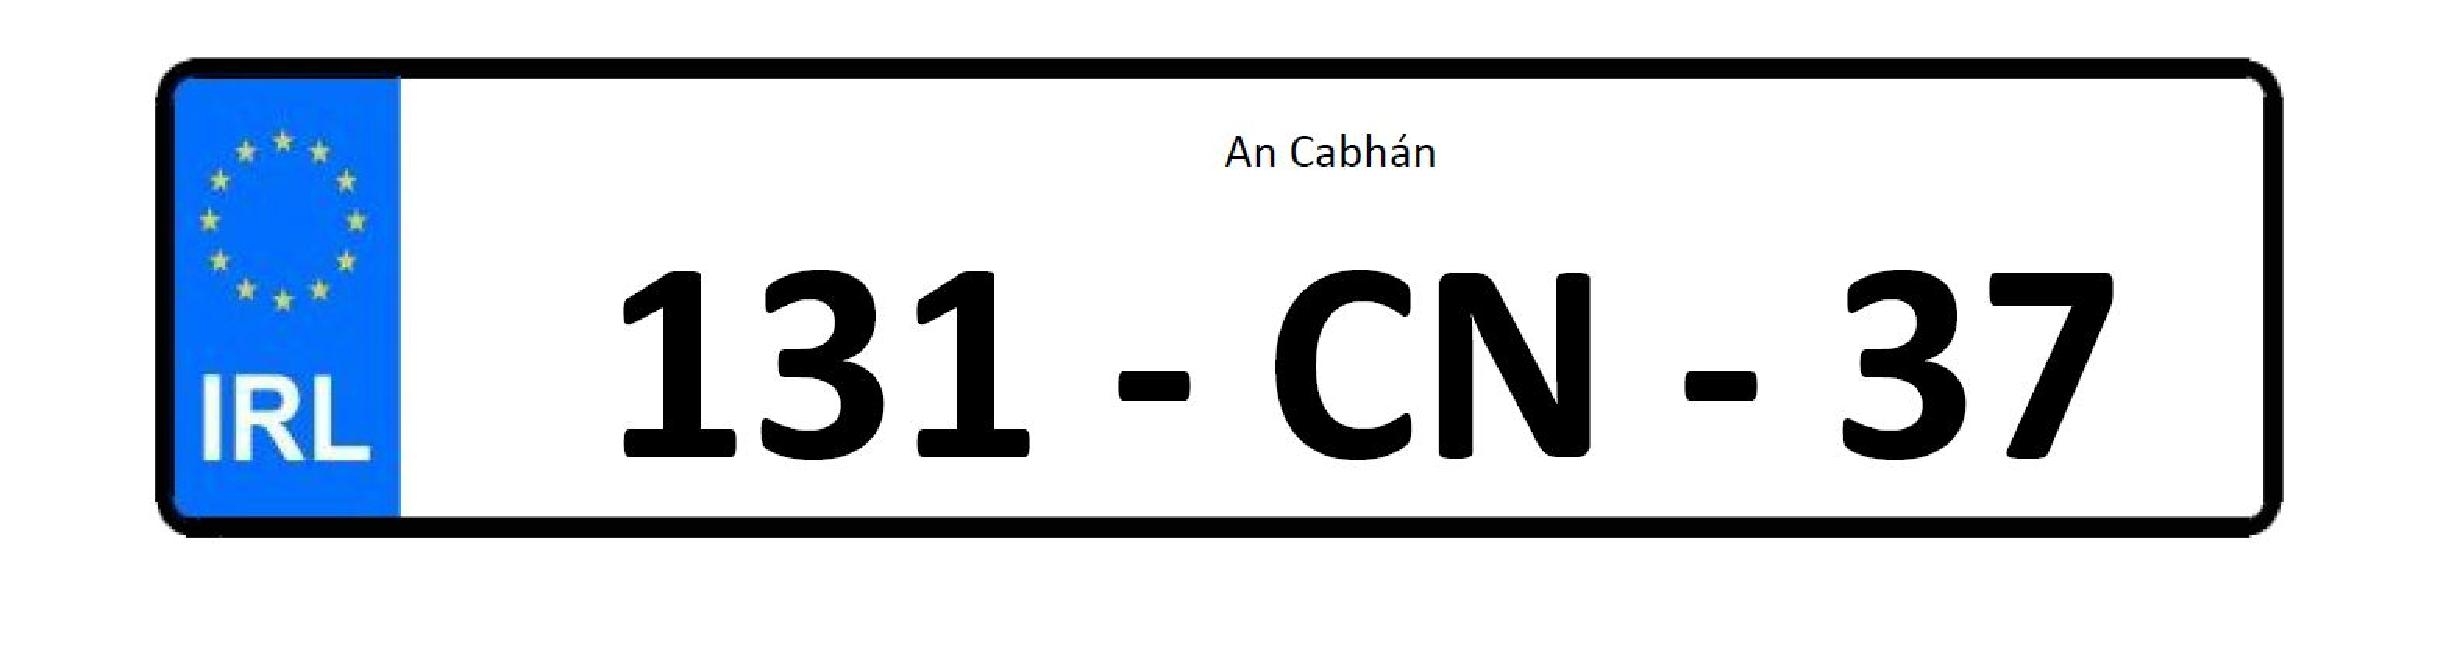
\includegraphics[height=1cm]{Results/Q2/NumPlate1/qanumber_plate_1.jpg}}%
		\subcaptionbox{Greyscale Image}
		[.3\linewidth]{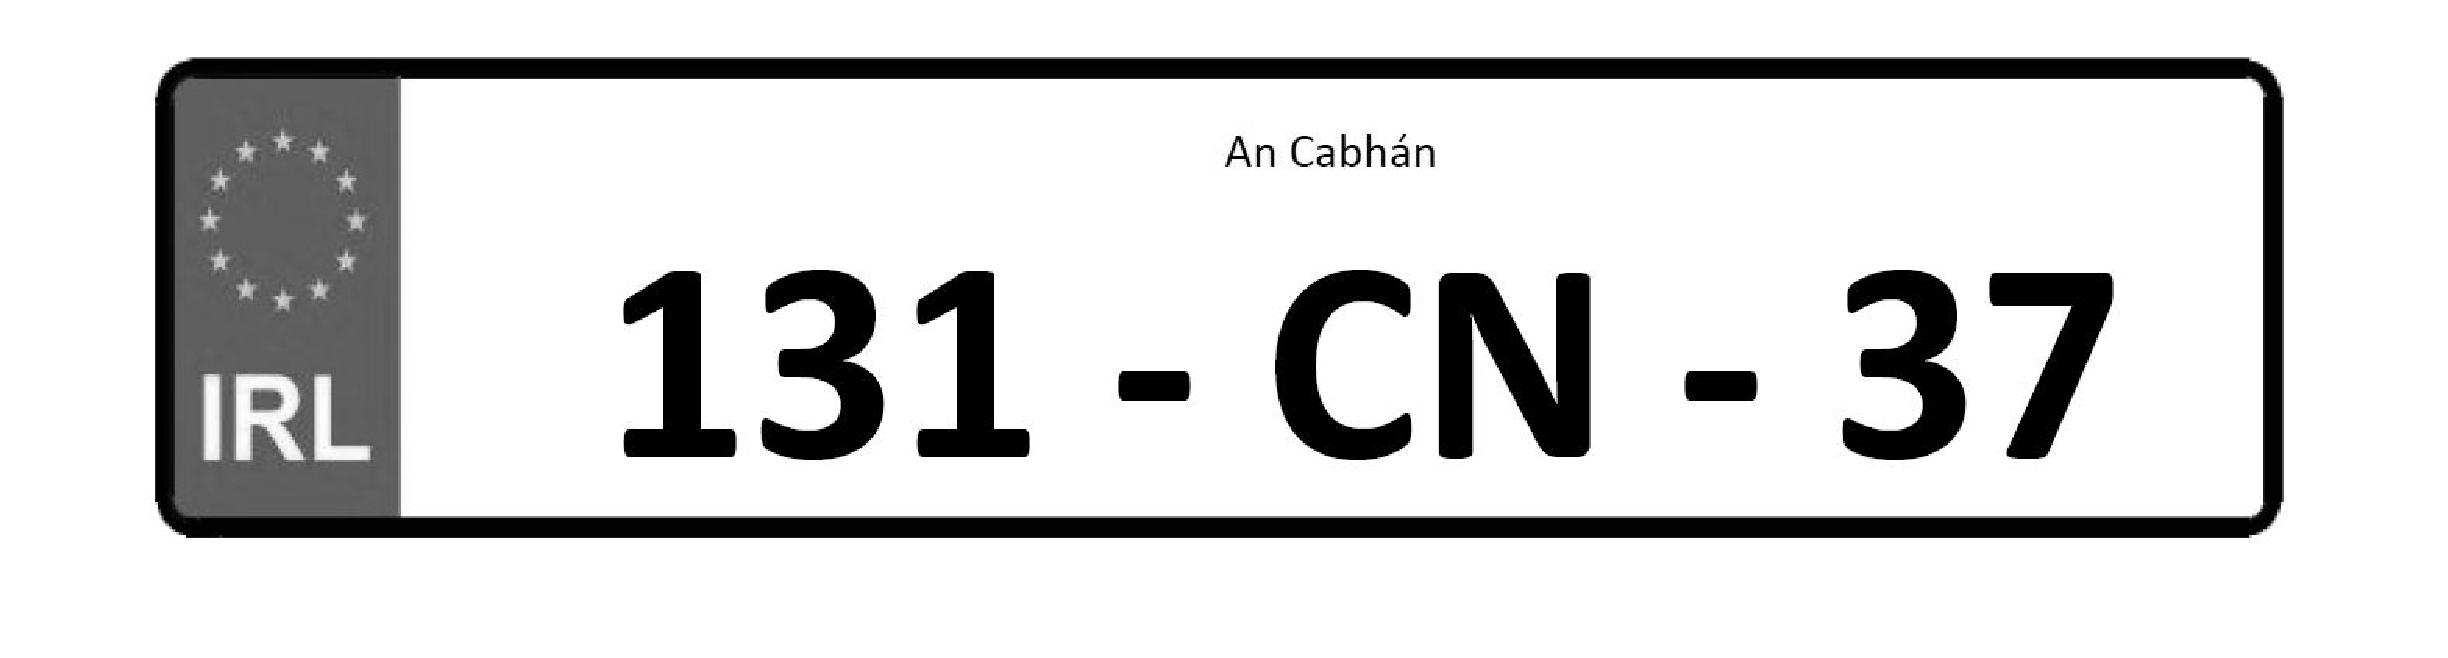
\includegraphics[height=1cm]{Results/Q2/NumPlate1/qanumber_plate_1Grey.jpg}}%
		\subcaptionbox{Low Pass Filtered}
		[.3\linewidth]{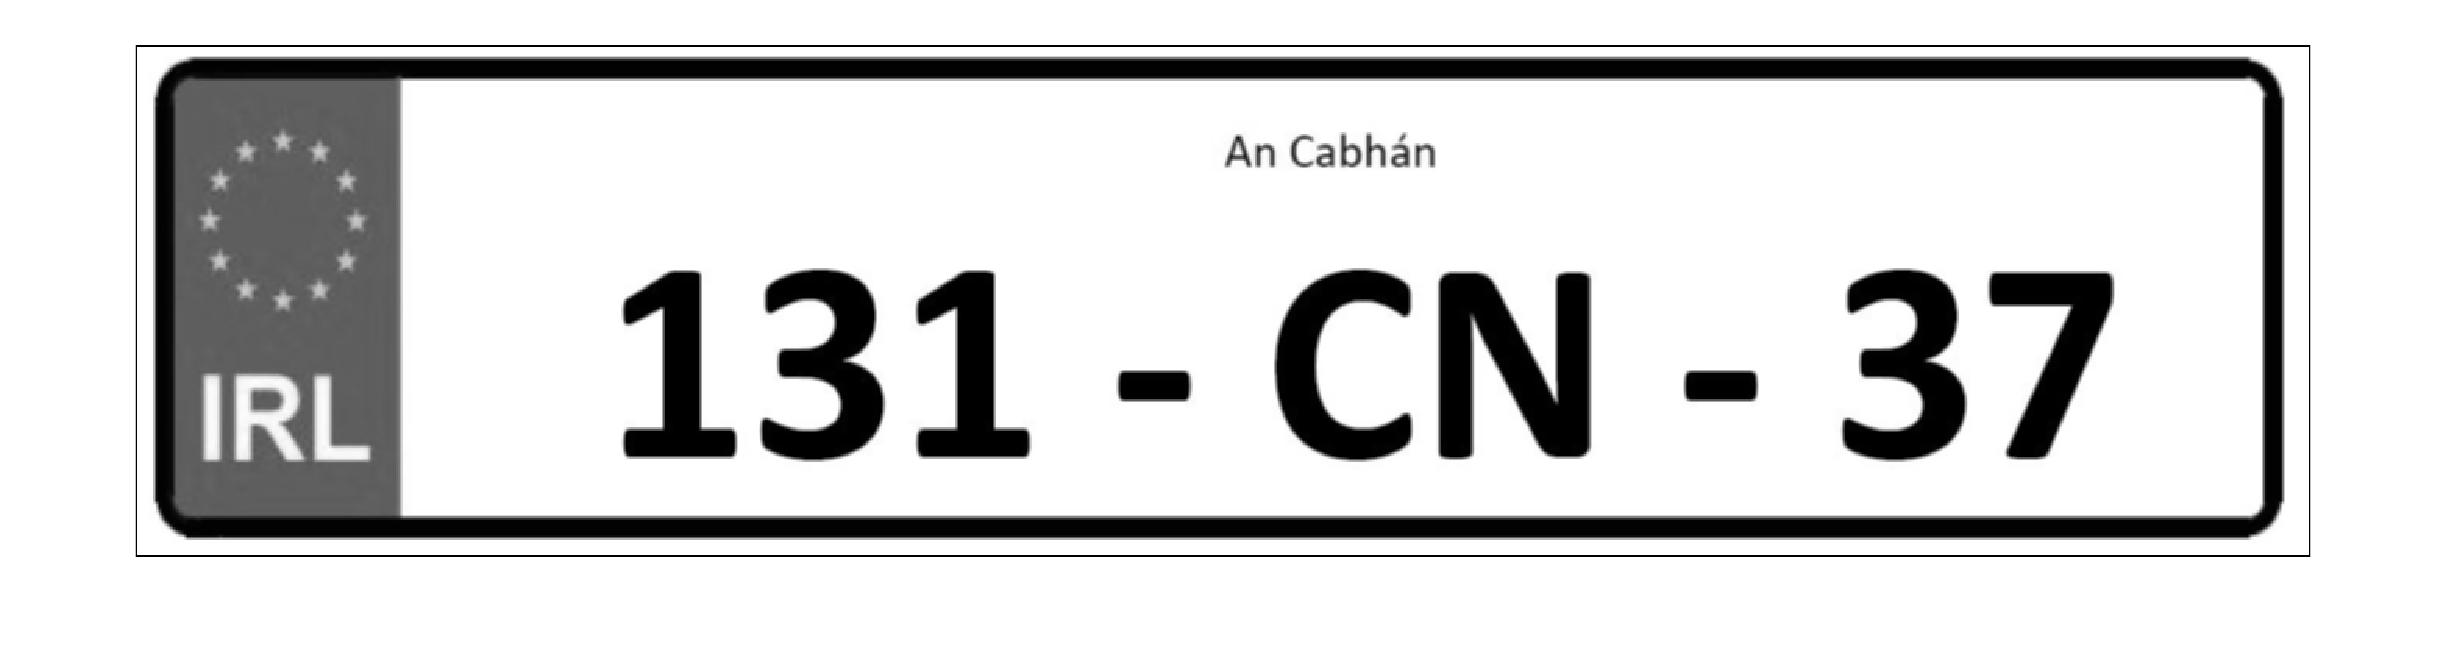
\includegraphics[height=1cm]{Results/Q2/NumPlate1/qanumber_plate_1Low.jpg}}%
		\caption{Initial Segmentation Setup}
		\label{fig:}
	\end{figure}
	\par The extraction process begins by applying a mid-value threshold to the
	image. The image is then inverted to allow for blob functions to be
	utilised. The border and country code are removed from the image by
	subtracting the biggest blob from the thresholded image.
	\begin{figure}[H]
		\centering
		\subcaptionbox{Mid Threshold}
		[.3\linewidth]{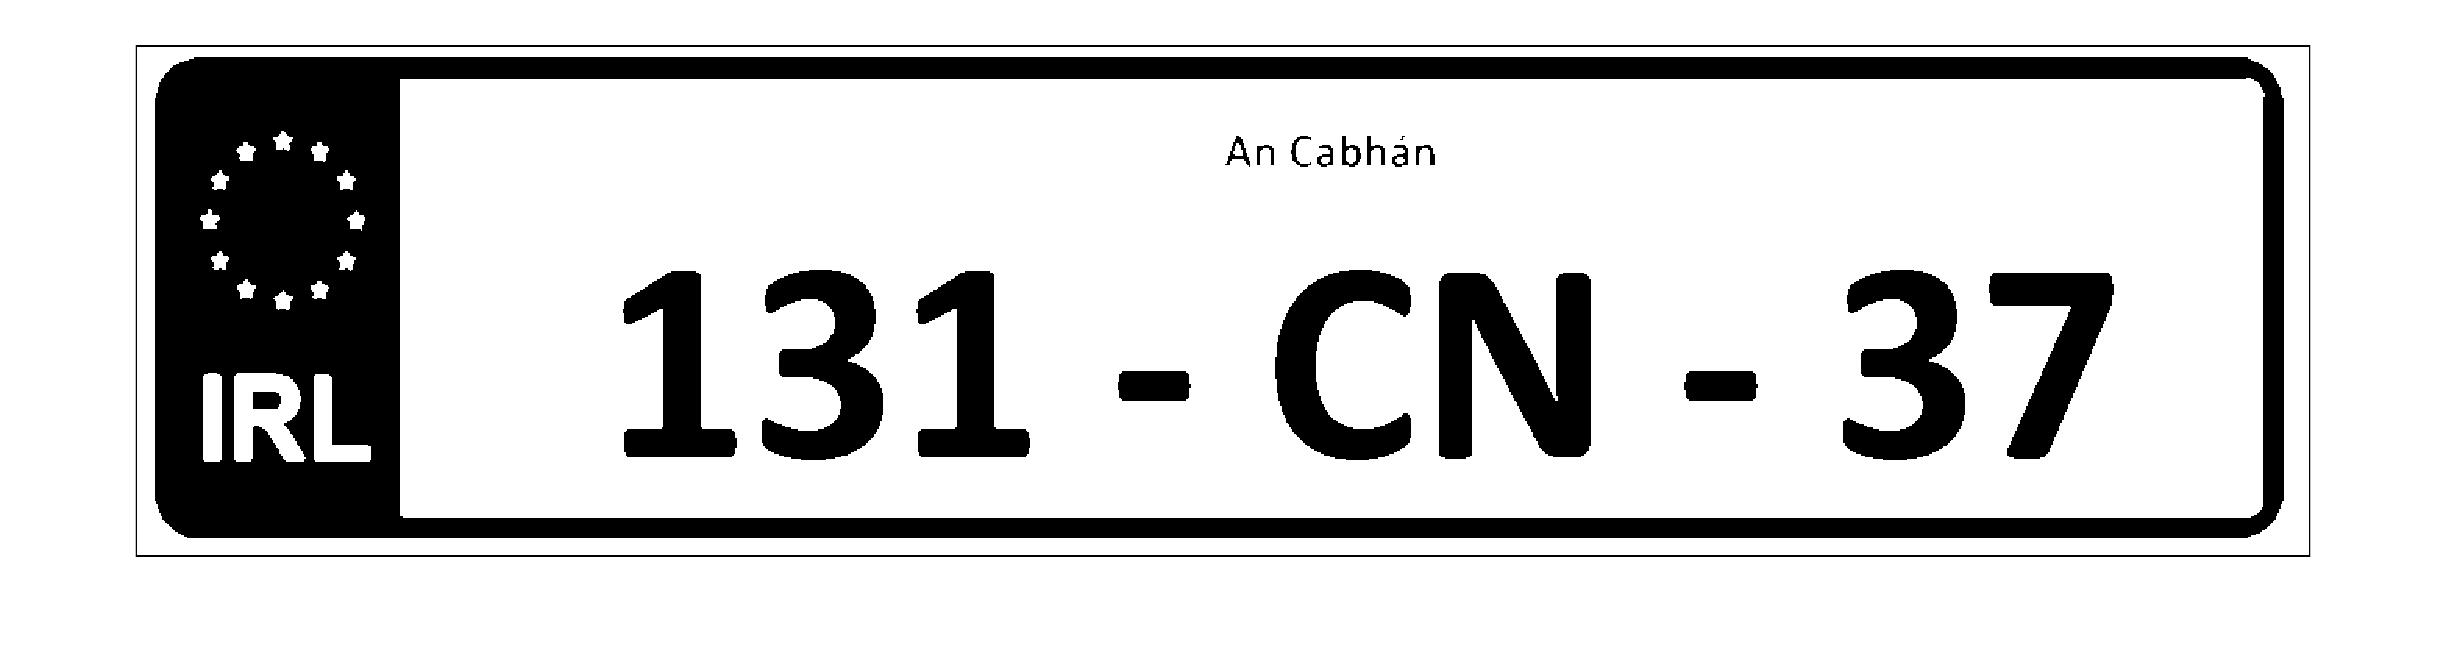
\includegraphics[height=1cm]{Results/Q2/NumPlate1/qanumber_plate_1Mid.jpg}}%
		\subcaptionbox{Inverted (Not)}
		[.3\linewidth]{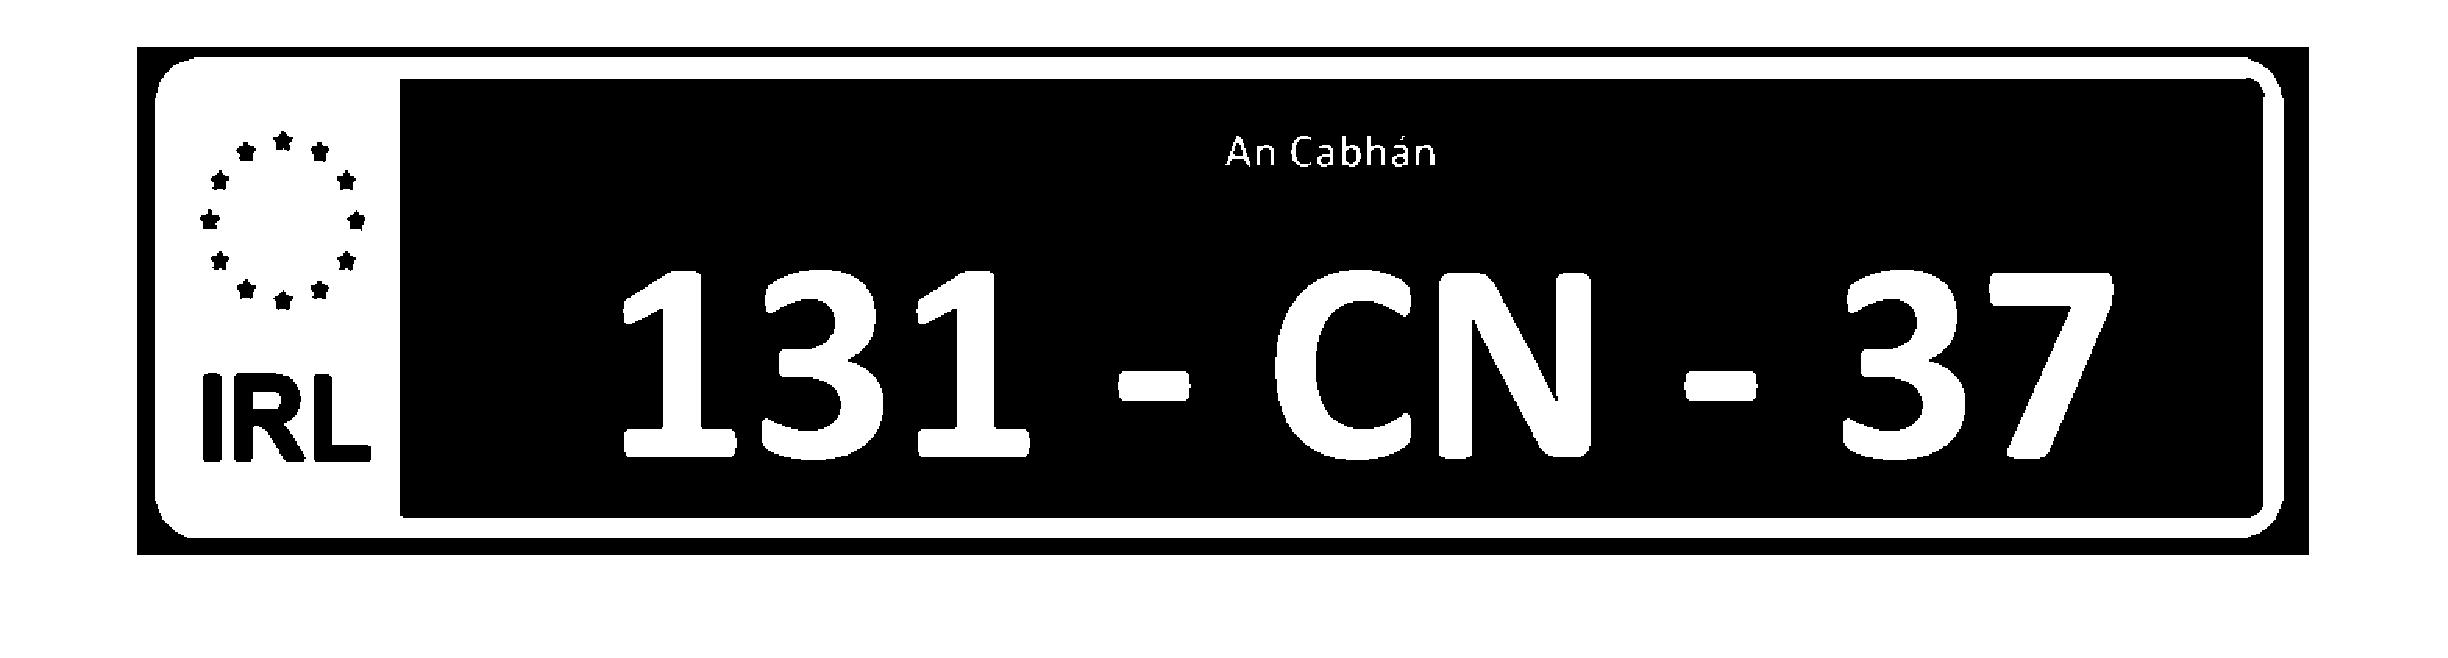
\includegraphics[height=1cm]{Results/Q2/NumPlate1/qanumber_plate_1Not.jpg}}%
		\caption{Preparing for Border Removal}
		\label{fig:}
	\end{figure}
	\begin{figure}[H]
		\centering
		\subcaptionbox{Biggest Blob}
		[.3\linewidth]{
\includegraphics[height=1cm]{Results/Q2/NumPlate1/qanumber_plate_1Border.jpg}}%
		\subcaptionbox{Biggest Blob Removed}
		[.3\linewidth]{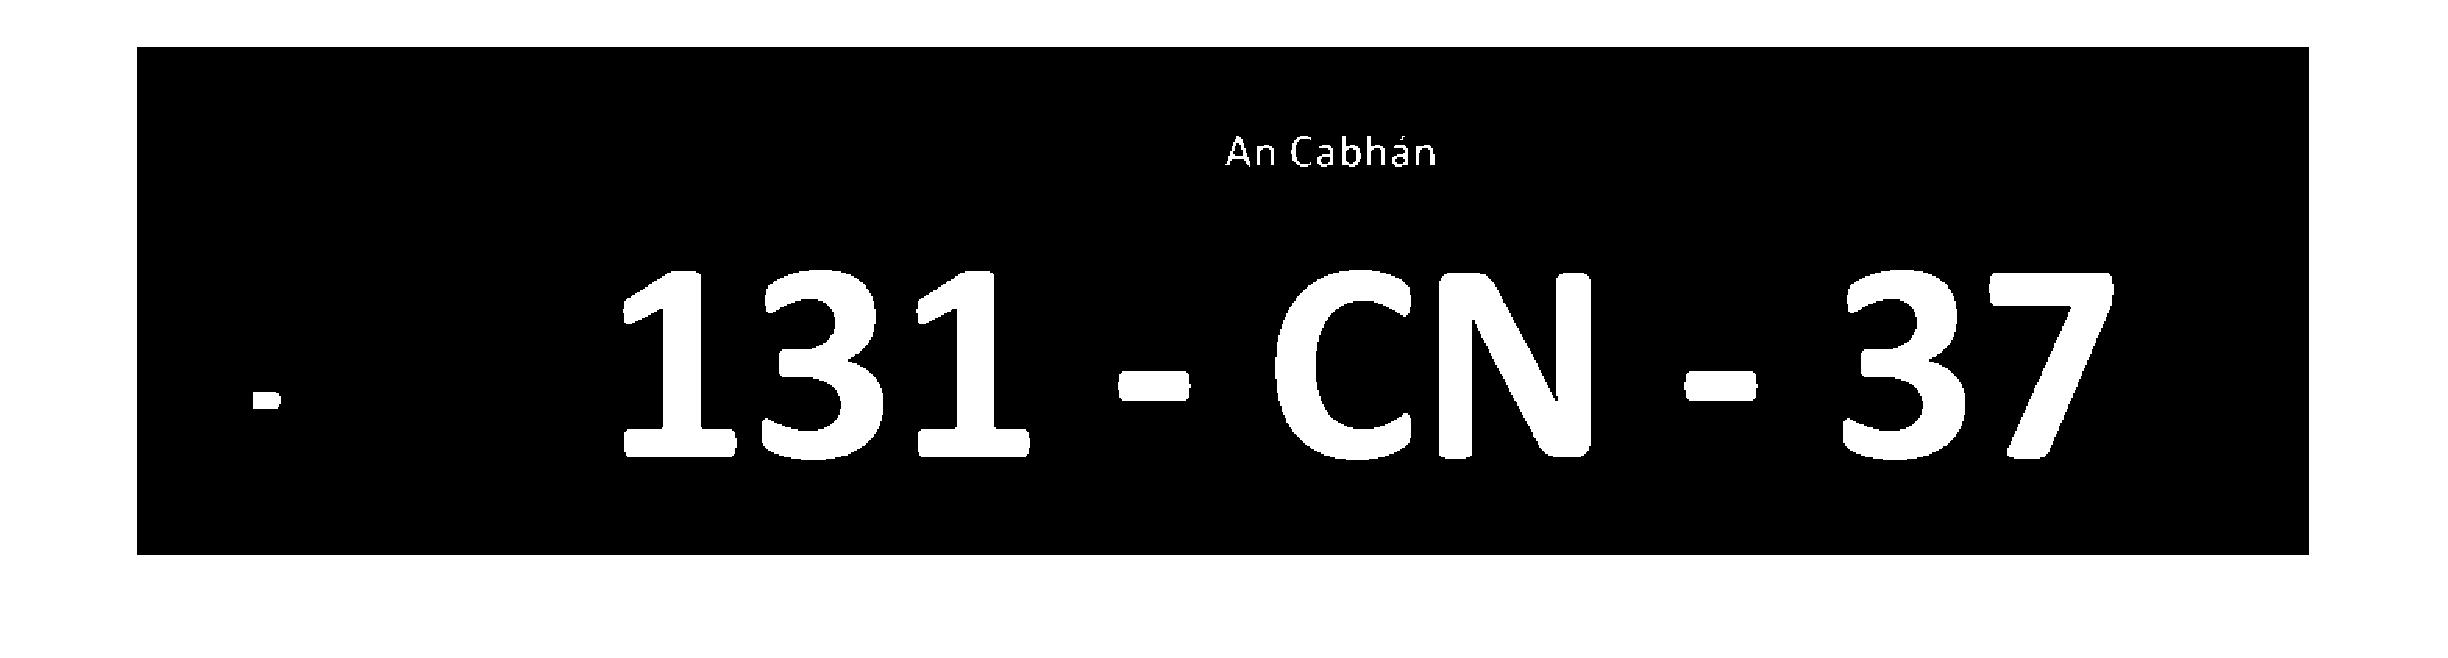
\includegraphics[height=1cm]{Results/Q2/NumPlate1/qanumber_plate_1NoBorder.jpg}}%
		\caption{Removed Outer Border}
		\label{fig:}
	\end{figure}
	\par Finally the main alphanumeric characters are extracted by looping
	through the blobs in the image, until the lower bound for the blob size
	is exceeded. The found blobs are then counted, and an edge detected
	version of the image is overlayed on the original image for display
	purposes.
	\begin{figure}[H]
		\centering
		\subcaptionbox{Largest Character}
		[.3\linewidth]{
\includegraphics[height=1cm]{Results/Q2/NumPlate1/qanumber_plate_1BigChar.jpg}}%
		\subcaptionbox{Remaining Characters}
		[.3\linewidth]{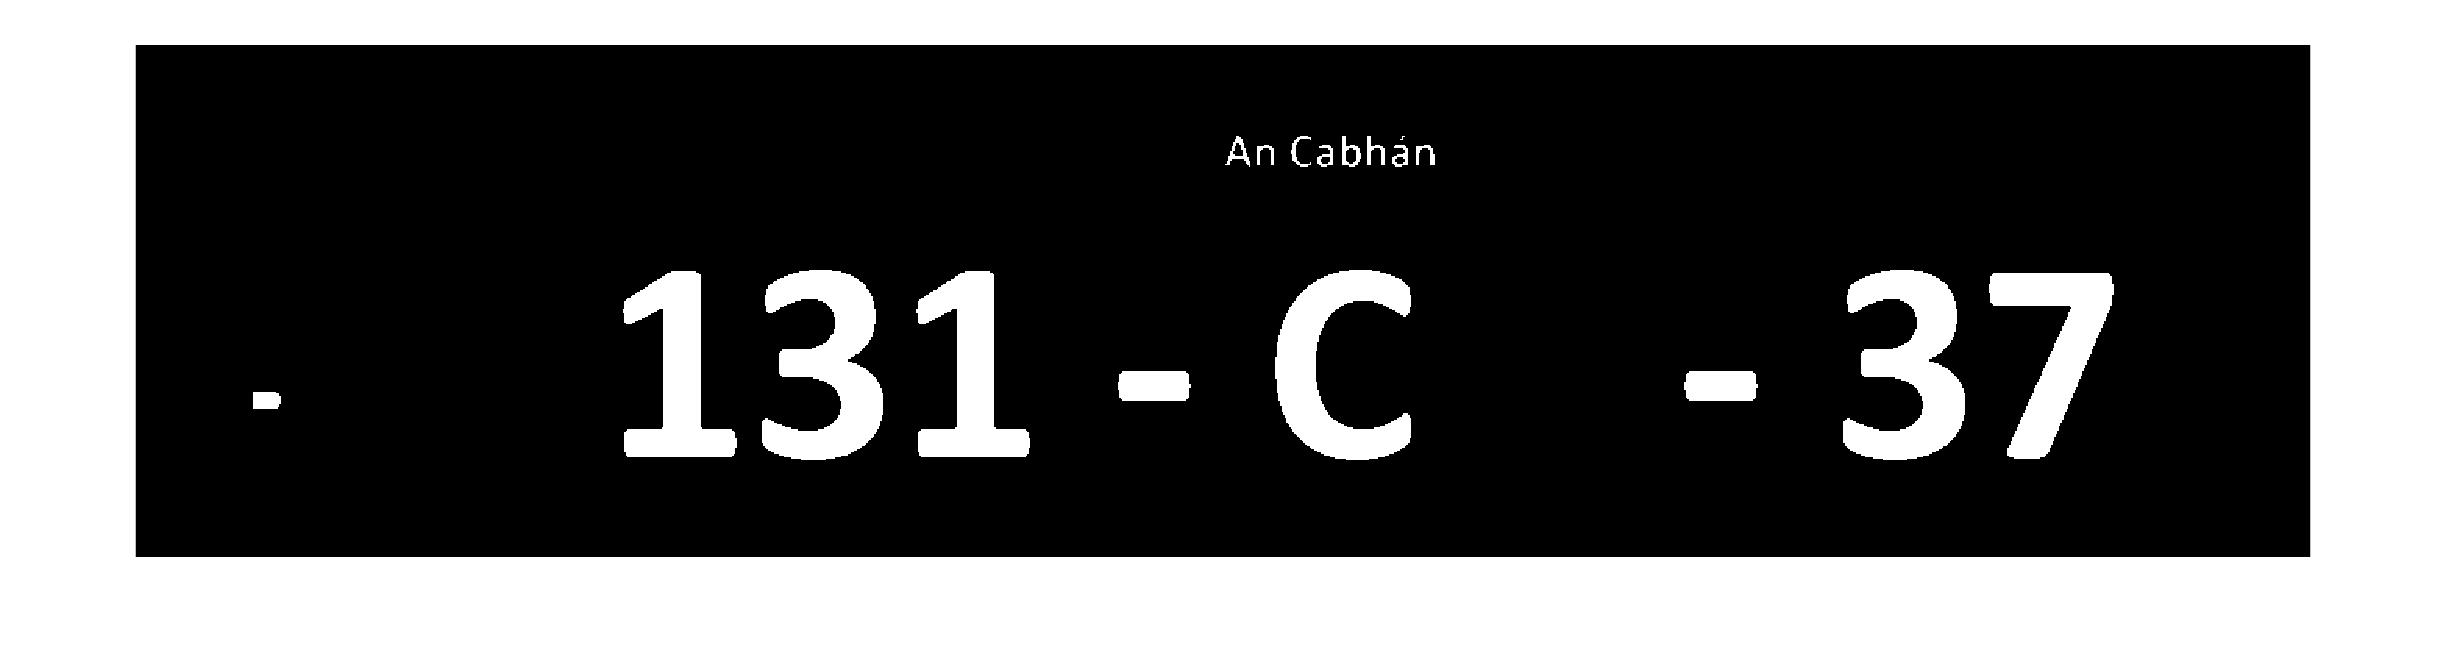
\includegraphics[height=1cm]{Results/Q2/NumPlate1/qanumber_plate_1Remain.jpg}}%
		\caption{Removed Largest Alphanumeric Character}
		\label{fig:}
	\end{figure}
	\begin{figure}[H]
		\centering
		\subcaptionbox{Loop 1 Result}
		[.3\linewidth]{
\includegraphics[height=1cm]{Results/Q2/NumPlate1/qanumber_plate_1Added1.jpg}}%
		\subcaptionbox{Loop 2 Result}
		[.3\linewidth]{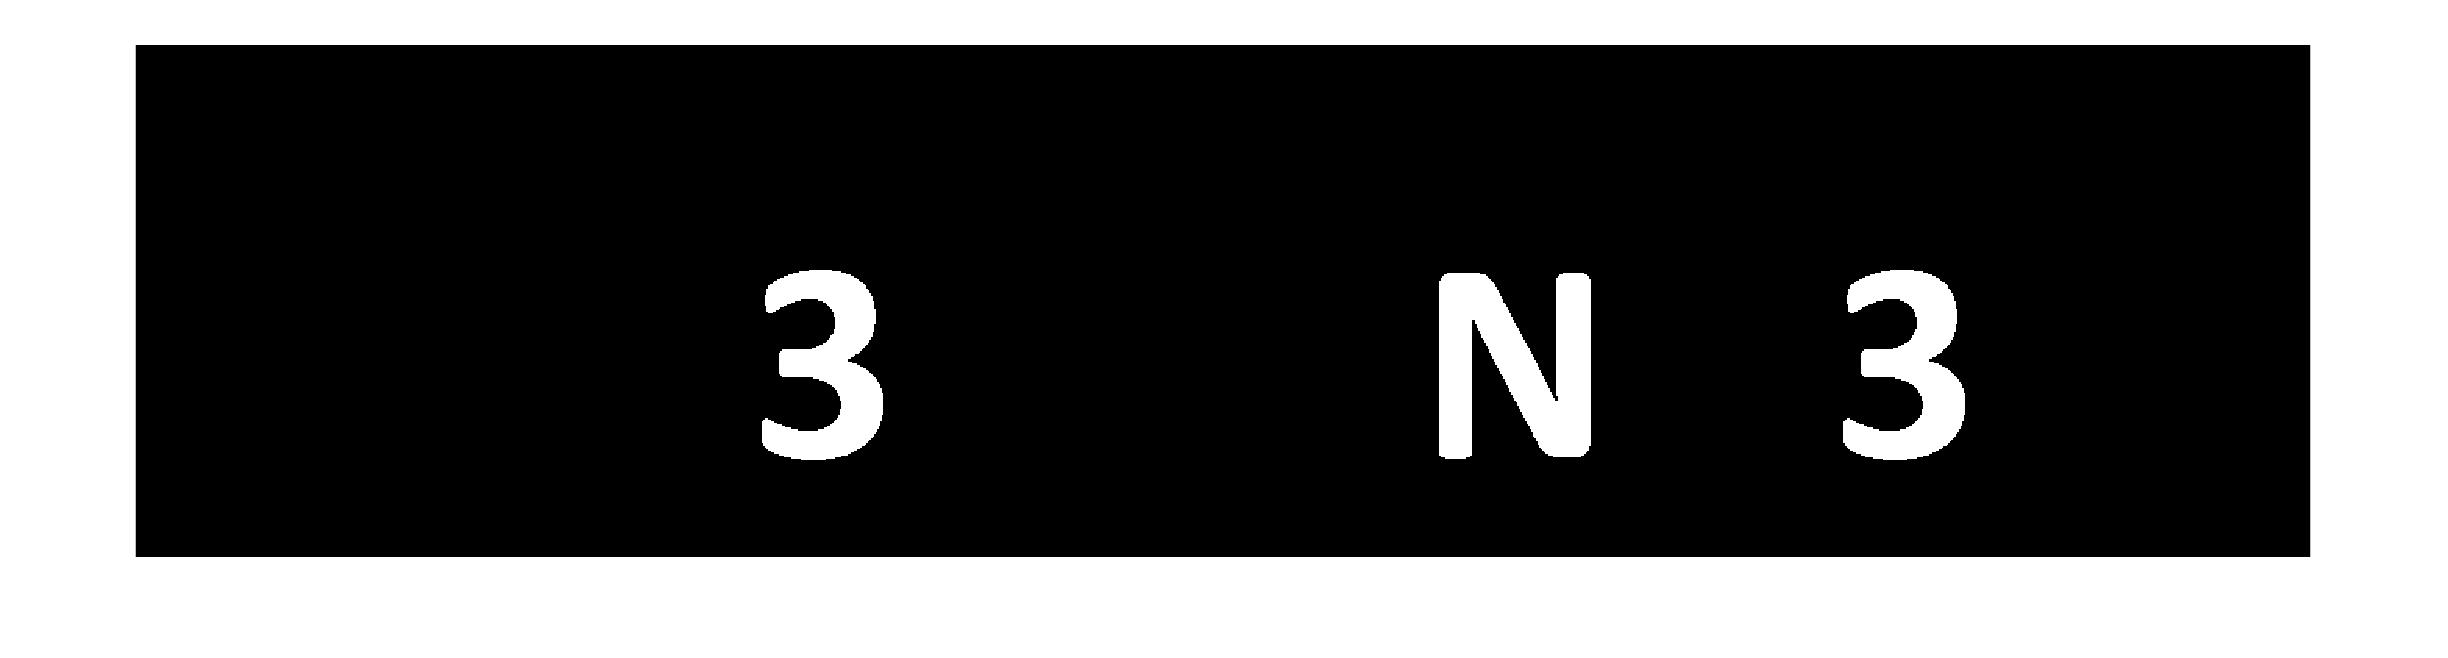
\includegraphics[height=1cm]{Results/Q2/NumPlate1/qanumber_plate_1Added2.jpg}}%
		\subcaptionbox{Loop 3 Result}
		[.3\linewidth]{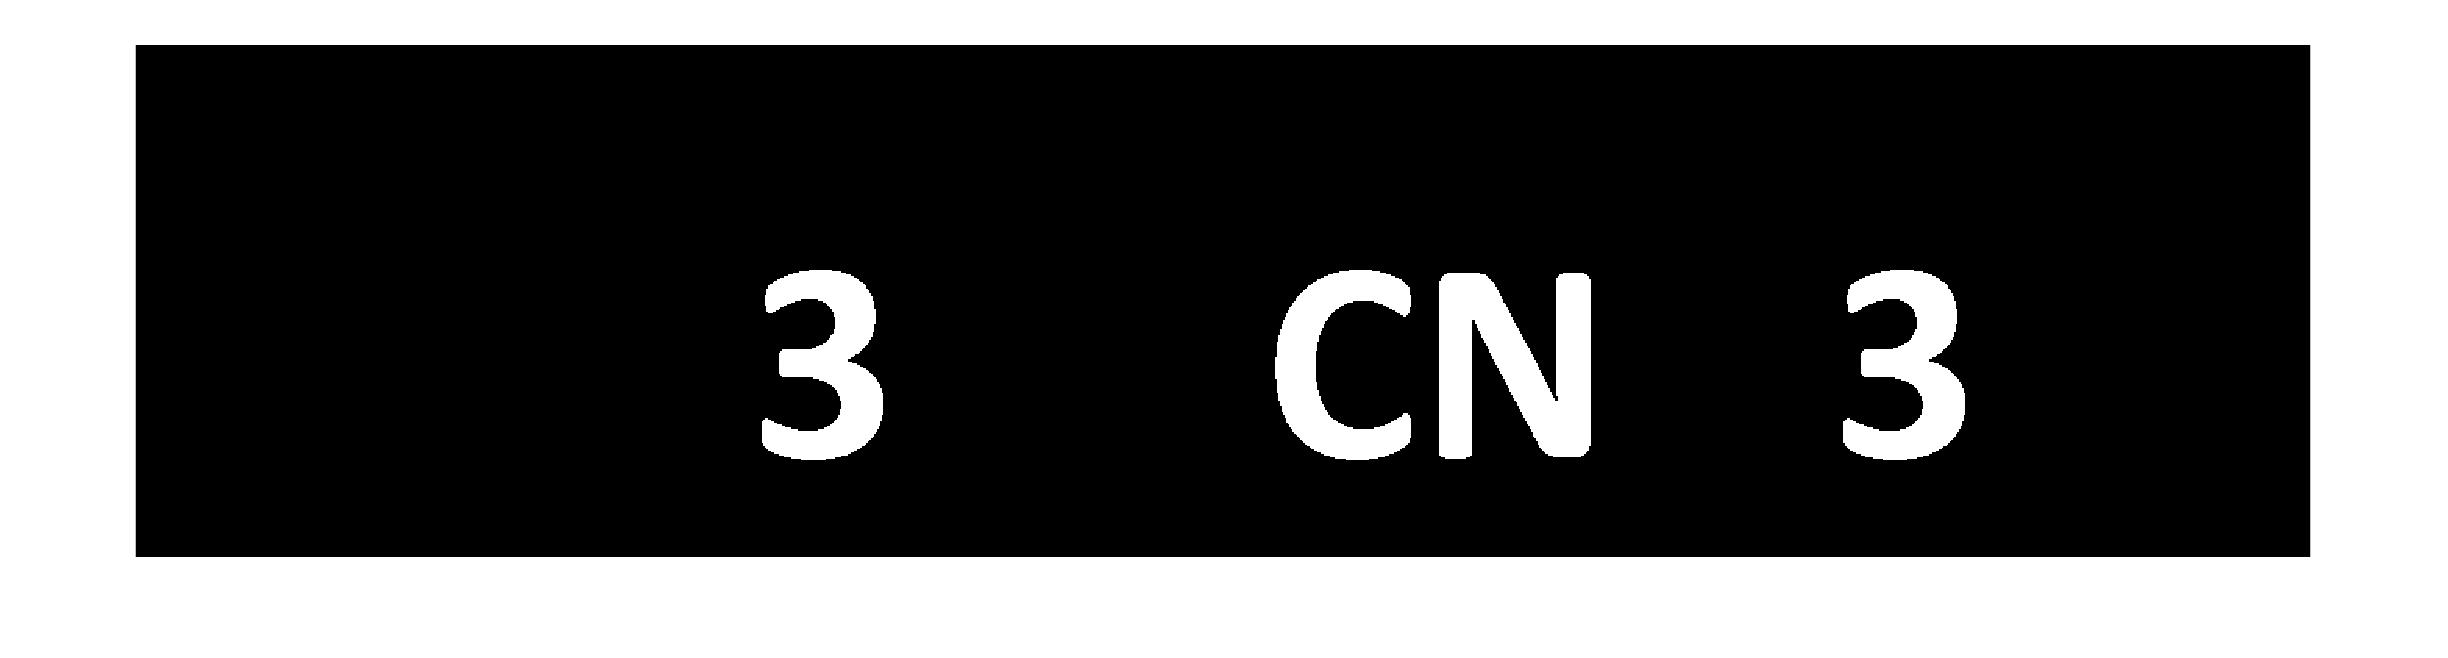
\includegraphics[height=1cm]{Results/Q2/NumPlate1/qanumber_plate_1Added3.jpg}}%
		\caption{Characters Extracted from Loops 1-3}
		\label{fig:}
	\end{figure}
	\begin{figure}[H]
		\centering
		\subcaptionbox{Loop 4 Result}
		[.3\linewidth]{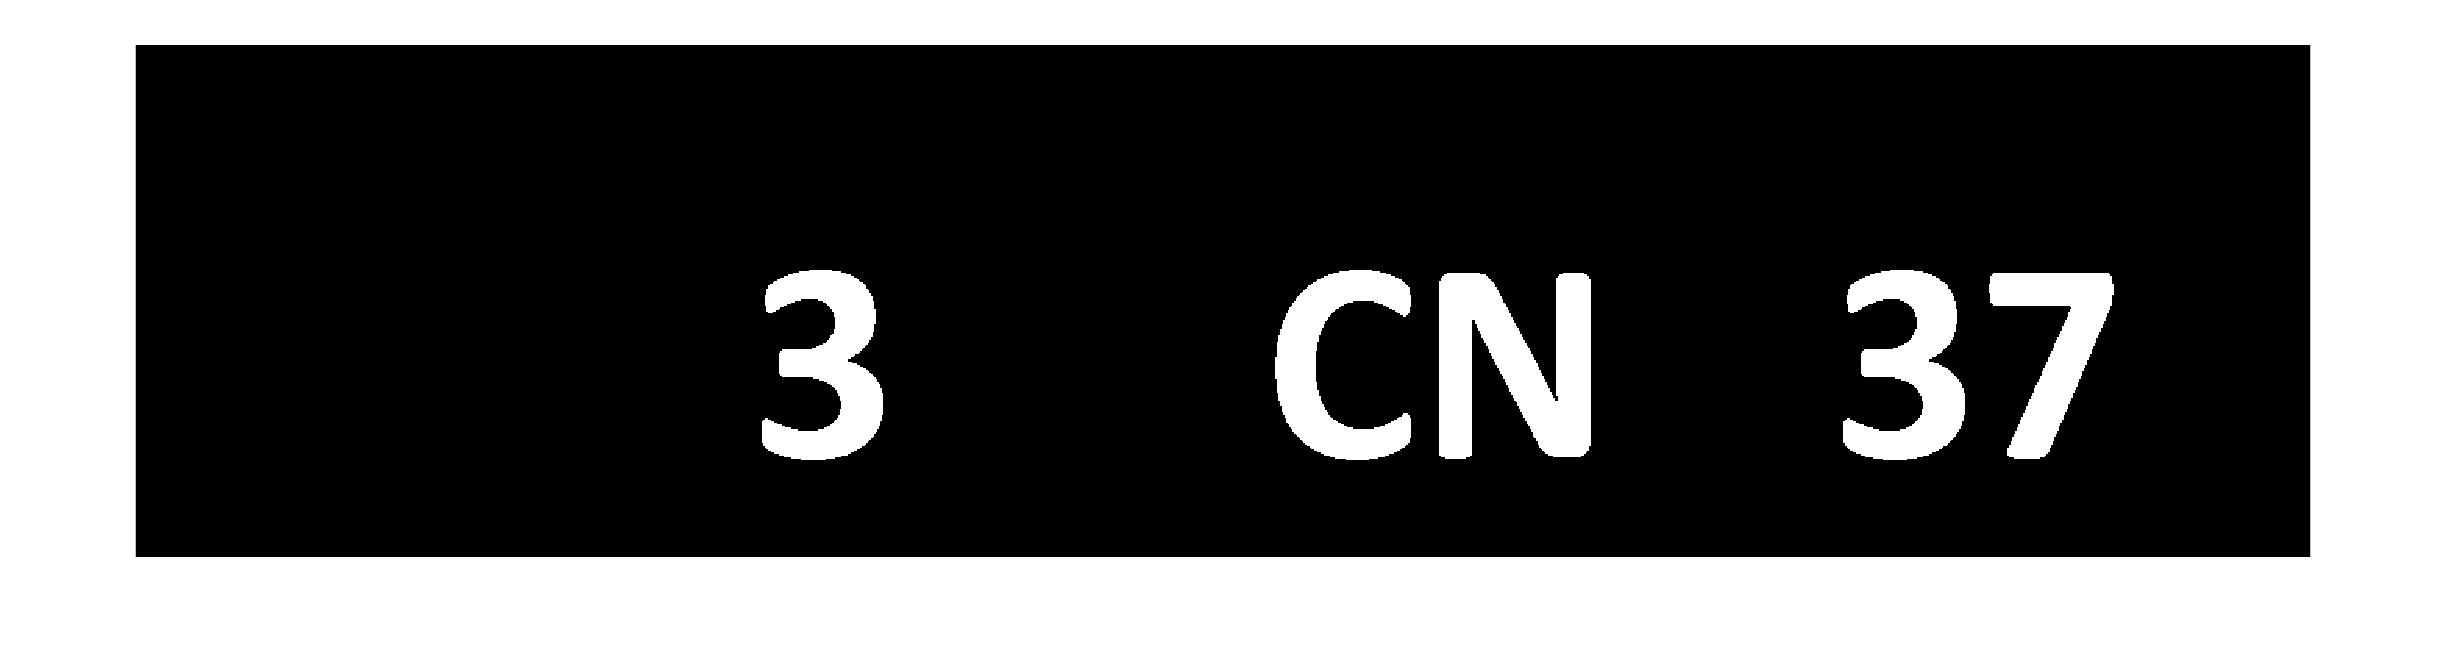
\includegraphics[height=1cm]{Results/Q2/NumPlate1/qanumber_plate_1Added4.jpg}}%
		\subcaptionbox{Loop 5 Result}
		[.3\linewidth]{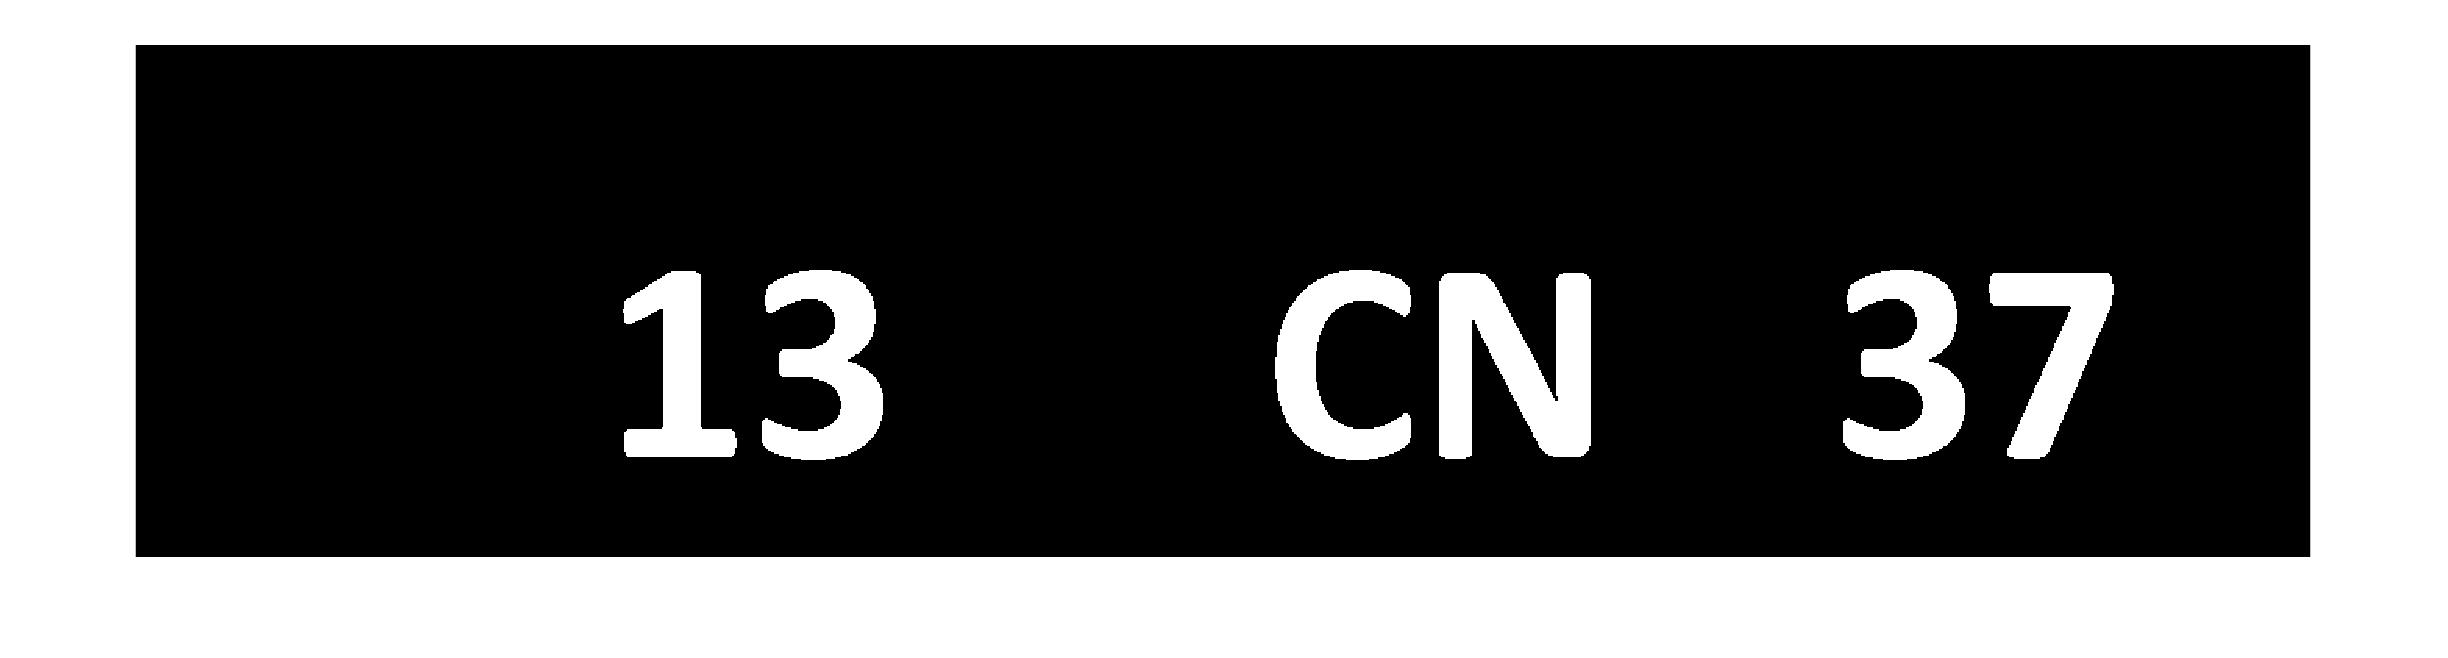
\includegraphics[height=1cm]{Results/Q2/NumPlate1/qanumber_plate_1Added5.jpg}}%
		\subcaptionbox{Loop 6 Result}
		[.3\linewidth]{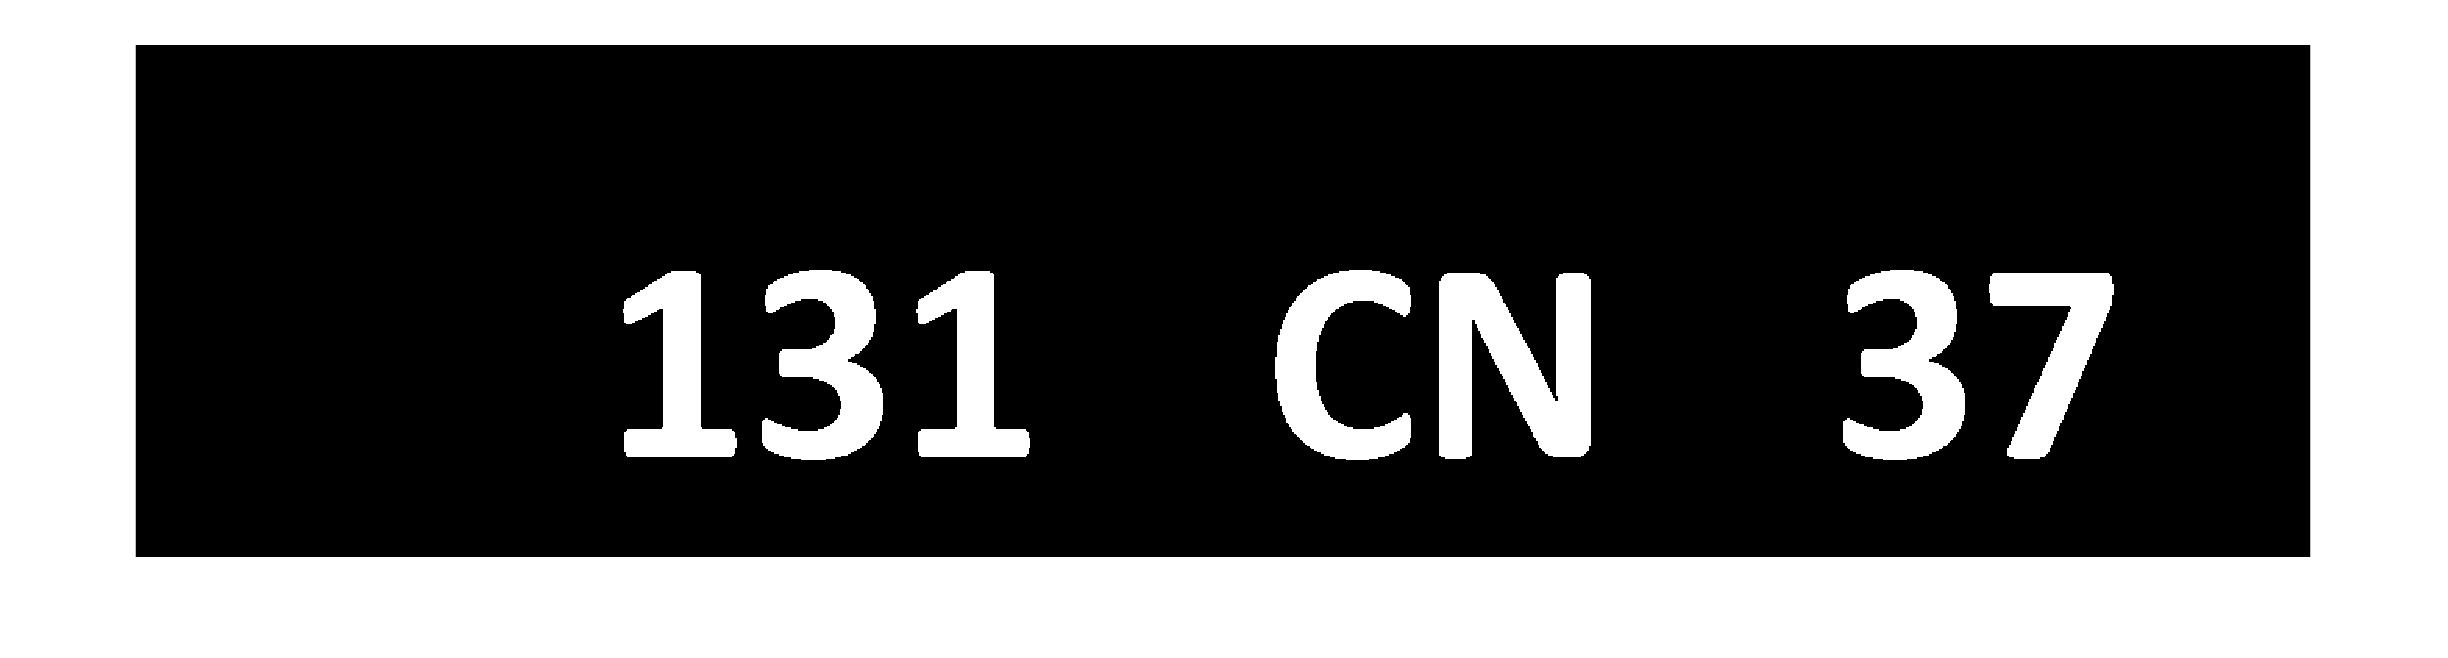
\includegraphics[height=1cm]{Results/Q2/NumPlate1/qanumber_plate_1Added6.jpg}}%
		\caption{Characters Extracted from Loops 4-6}
		\label{fig:}
	\end{figure}
	\begin{figure}[H]
		\centering
		\subcaptionbox{Canny Edge Detection}
		[.4\linewidth]{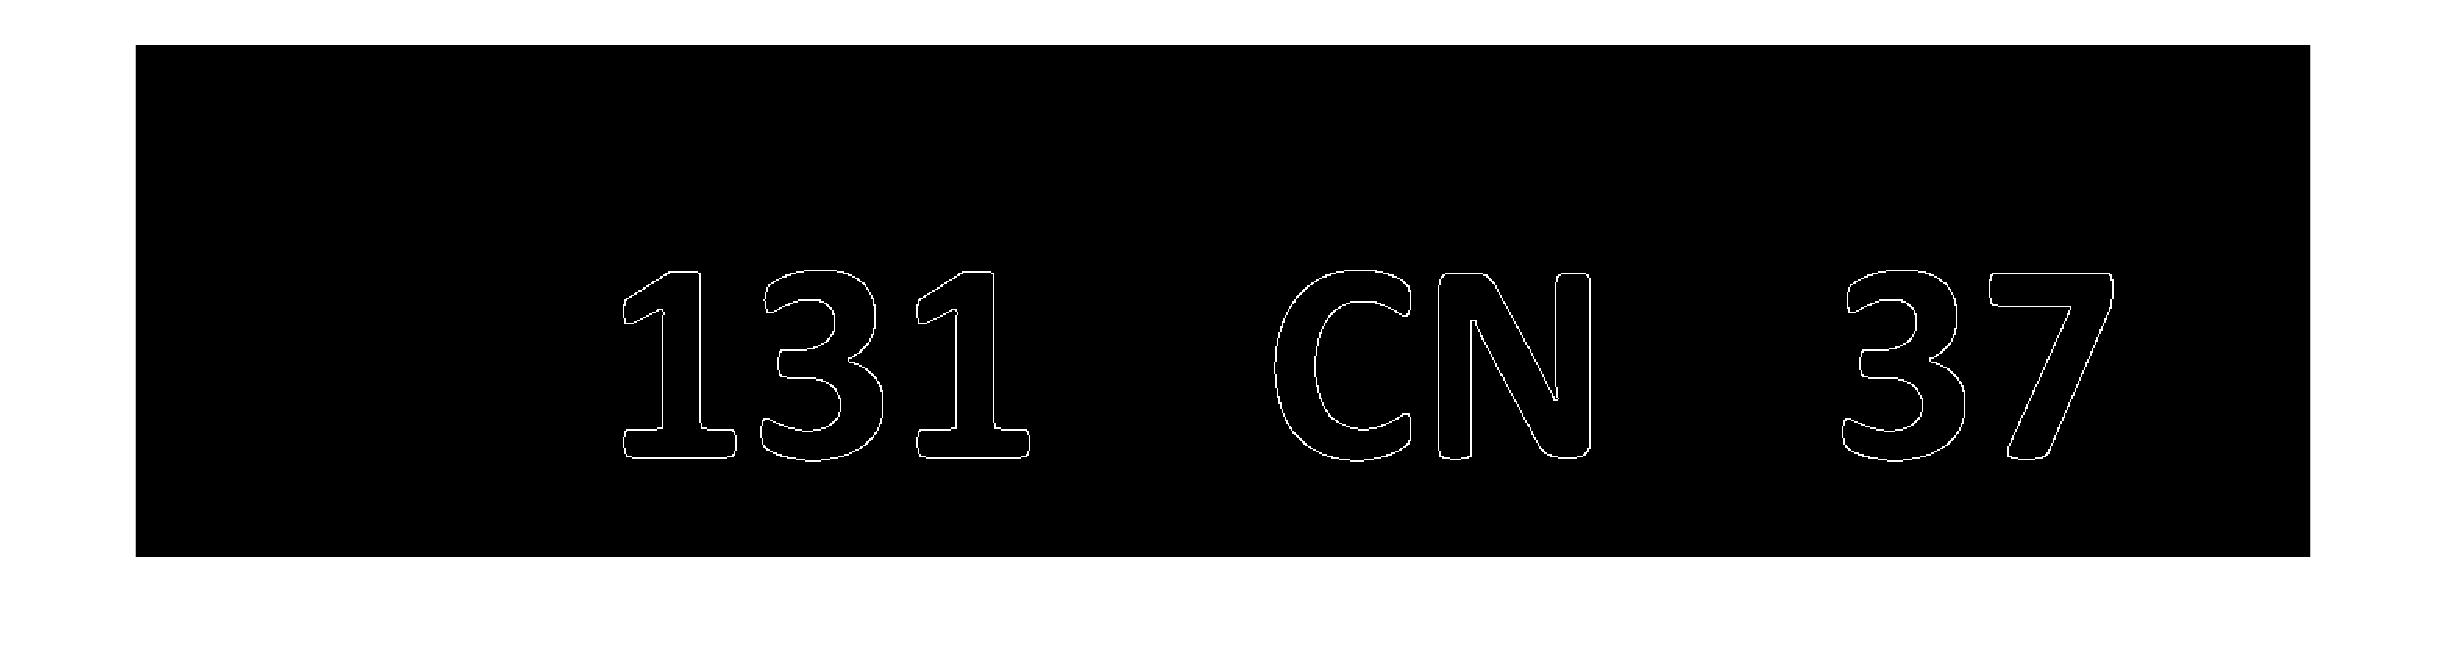
\includegraphics[height=1.25cm]{Results/Q2/NumPlate1/qanumber_plate_1Canny.jpg}}%
		\subcaptionbox{Overlayed Images}
		[.4\linewidth]{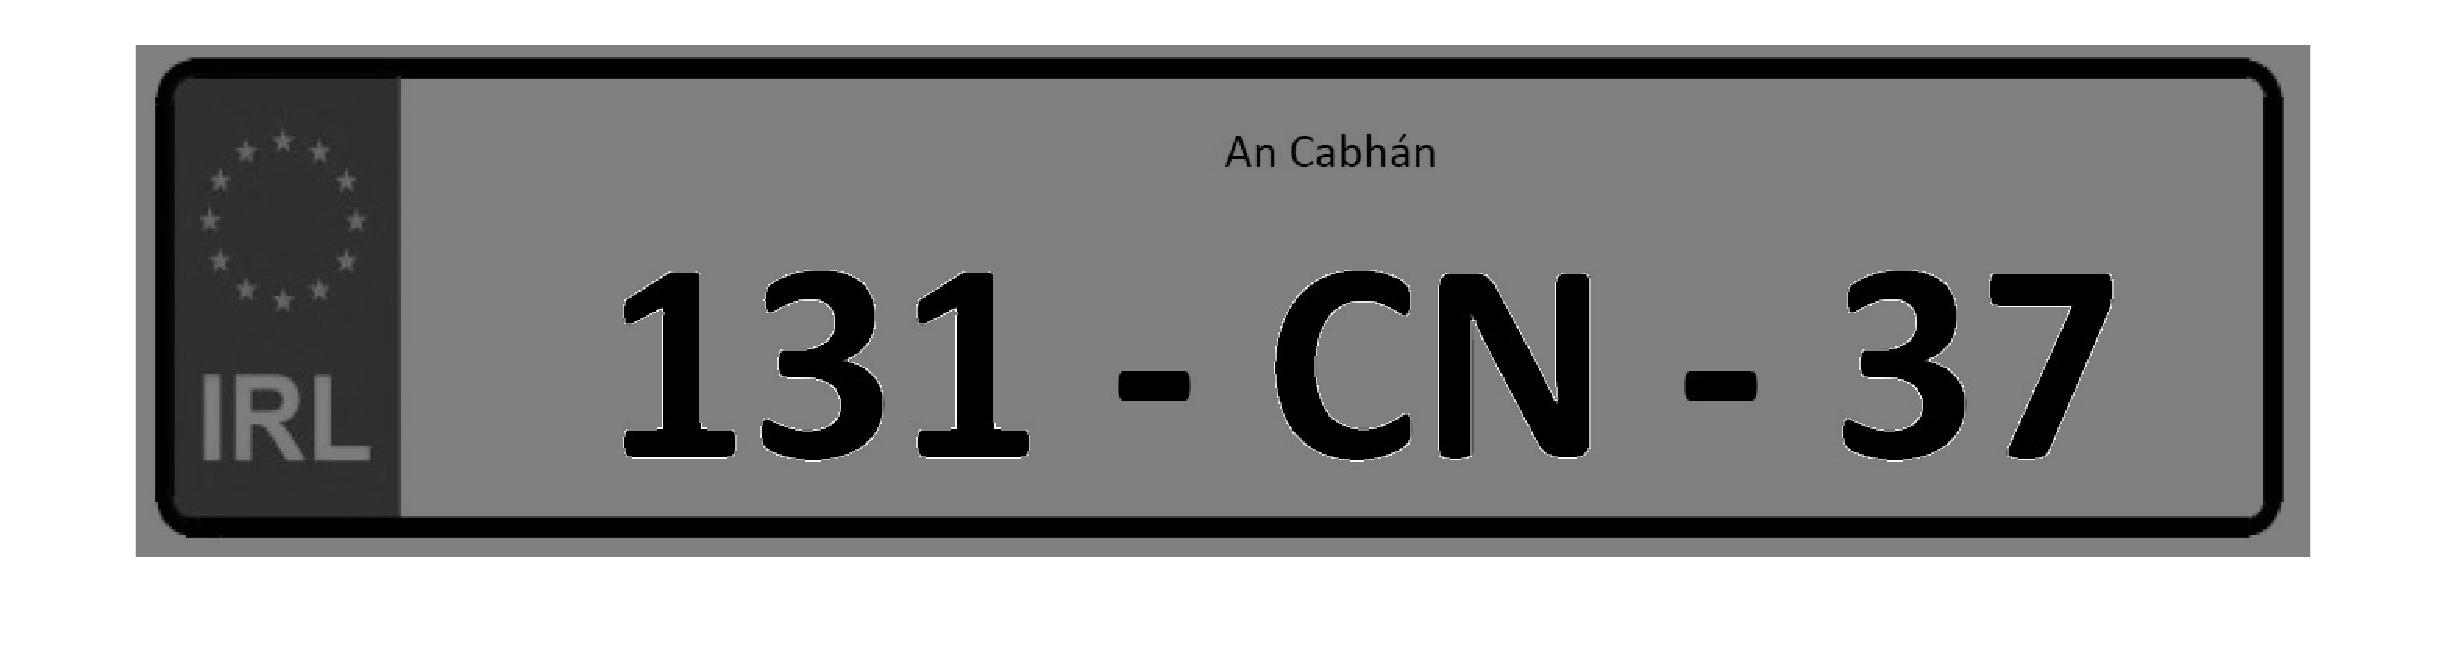
\includegraphics[height=1.25cm]{Results/Q2/NumPlate1/qanumber_plate_1Overlay.jpg}}%
		\caption{Overlayed Extracted Characters}
		\label{fig:}
	\end{figure}
	\par In order to test that this code is working as intended, a unit test file
	(q2patest.m) is executed. The original .m file is converted to a
	function, with the output being the number of characters found. An
	assertion within the unit test checks each test licence plate image
	against it's expected resulting number of characters.
	\subsubsection{Part b}
	\subsection{Conclusion}
	\section{Part 3: Convolution}
	\subsection{Introduction}
	\subsection{Techniques}
	\subsection{Pseudocode}
	\subsubsection{Part a}
	\begin{enumerate}
		\item Load the image into Matlab using the ``imread()''
			function.
		\item Use the ``rgb2gray()'' function to convert the image to
			greyscale.
		\item Load the template image into Matlab using the ``imread()''
			function.
		\item Use the ``rgb2gray()'' function to convert the image to
			greyscale.
	\end{enumerate}
	\subsection{Results}
	\subsubsection{Part a}
	\subsubsection{Part b}
	\subsubsection{Part c}
	\subsection{Conclusion}
	\section{Appendix}
	\subsection{Part 1:}
	\subsubsection{Code:}
	\subsection{Part 2:}
	\subsubsection{Code:}
	\subsubsection{Images:}
	\subsection{Part 3:}
	\subsubsection{Code:}
	\subsubsection{Images:}
\end{document}
